\documentclass[11pt]{article}
\usepackage{fullpage}
\usepackage{graphicx}
\usepackage{hyperref}
\usepackage{fixltx2e}
\usepackage{amsmath}
\usepackage{mathtools}
\usepackage{xcolor}
\usepackage{listings}
\usepackage{minted}
\usepackage{todonotes}
\usepackage{lscape}
\usepackage{tabularx}
\lstset{
    frame=single,
    breaklines=true,
    postbreak=\raisebox{0ex}[0ex][0ex]{\ensuremath{\color{blue}\hookrightarrow\space}}
}
\renewcommand{\abstractname}{\vspace{-\baselineskip}}
\begin{document}
\title{%
	EUTelescope: User Guide\\
    \large Version 1.0.0
}
\date{\today}
\author{Tom Daubney et al. on behalf of the EUTelescope Development Team}
\maketitle
\begin{abstract}
This guide covers the installation and basic operation of EUTelescope. It is composed of an edited selection of resources already available on the web, as well as new content and examples that have not been documented before. It is my hope that this guide will improve with age as I will be releasing the guide on an iterative basis with the intention of keeping it as up-to-date and error free as possible.\\

Should you find any mistakes in the guide, or feel that something important is missing, please log it with the EUTelescope issue tracker at \url{https://github.com/eutelescope/eutelescope/issues} and I will include it in my next update.
\end{abstract}
\newpage
\tableofcontents
\newpage
\section{Introduction}
\paragraph{}
This guide is intended for all users of EUTelescope. It is an all inclusive guide covering the installation process to the operation, right the way through to troubleshooting. This guide can be read all in one go, if one has the inclination, or it can be dipped in and out of to revise procedures as and when the user sees fit.
\paragraph{}
Please, whilst working through this guide, pay special attention to the portions of the guide where carriage return arrows ($\hookrightarrow$) appear in bash commands. This is purely \LaTeX\  indicating that the command is too long for one line. When entering the command into your terminal, please ignore the arrow.\\ \\
If you notice any errors in this guide, please contact Tom Daubney: \textit{thomas.daubney@desy.de}. 
\subsection{Overview}
\paragraph{•}
The EUTelescope[1] framework is a group of Marlin (link is external) processors that are used for the analysis and reconstruction of data taken with pixel beam telescopes. It was implemented in the context of the EUDET project supported by the European Union in its 6th Framework Programme for the European Research Area, and is embedded into the ILCsoft framework. The main goal of the EUTelescope software is to get from raw data to high level objects like tracks crossing through the telescope. These tracks are used to characterize both the telescope itself and any other position sensitive detector (DUT =``device under test'') that can be inserted into the telescope setup.
\paragraph{•}
The EUTelescope software package was originally created as consistent data analysis chain for the EUDET telescopes. These telescopes consist of six planes with high-resolution MIMOSA26 pixel sensors and are constructed to provide a full-featured infrastructure for DUT measurements. This includes the telescope with the sensors, cooling, and readout electronics as well as the Data Acquisition (DAQ) tool EUDAQ and the analysis software EUTelescope. The ILCsoft framework is being developed by the ILC community and unites several tools for data processing, originally intended for application in detector development efforts towards the International Linear Collider (ILC). The core elements of the framework are the Linear Collider I/O (LCIO) data model, the Geometry API for Reconstruction (GEAR) markup language and the event processor Modular Analysis \& Reconstruction for the LINear collider (Marlin).
\paragraph{•}
The implementation of EUTelescope into the ILCsoft framework and its modular structure has several advantages, such as the possibility to submit large analysis jobs for Grid computing and the possibility of a simple step-by-step analysis chain. Marlin allows the modular composition of analysis chains for various applications. Every task is implemented as an independent processor that is called by Marlin. The processors can expose parameters to the user which can be configured and loaded at runtime via so-called steering files in Extensible Markup Language (XML) format.
\paragraph{•}
The main input of the full analysis chain is the LCIO output file produced by the DAQ system containing the pixel raw data. Along with that other data is also needed: for example calibration constants (pedestal and noise), eta distributions for each sensor and alignment constants. EUTelescope provides several processors for Marlin implementing algorithms necessary for a full track reconstruction and data analysis of beam test experiments. Most of the EUTelescope processors have been developed for the full-frame readout MIMOSA26 sensors and later adapted for zero-suppressed data. ILCsoft and EUTelescope installations are available on the DESY Andrew File System (AFS).
\begin{figure}[!ht]
	\centering
	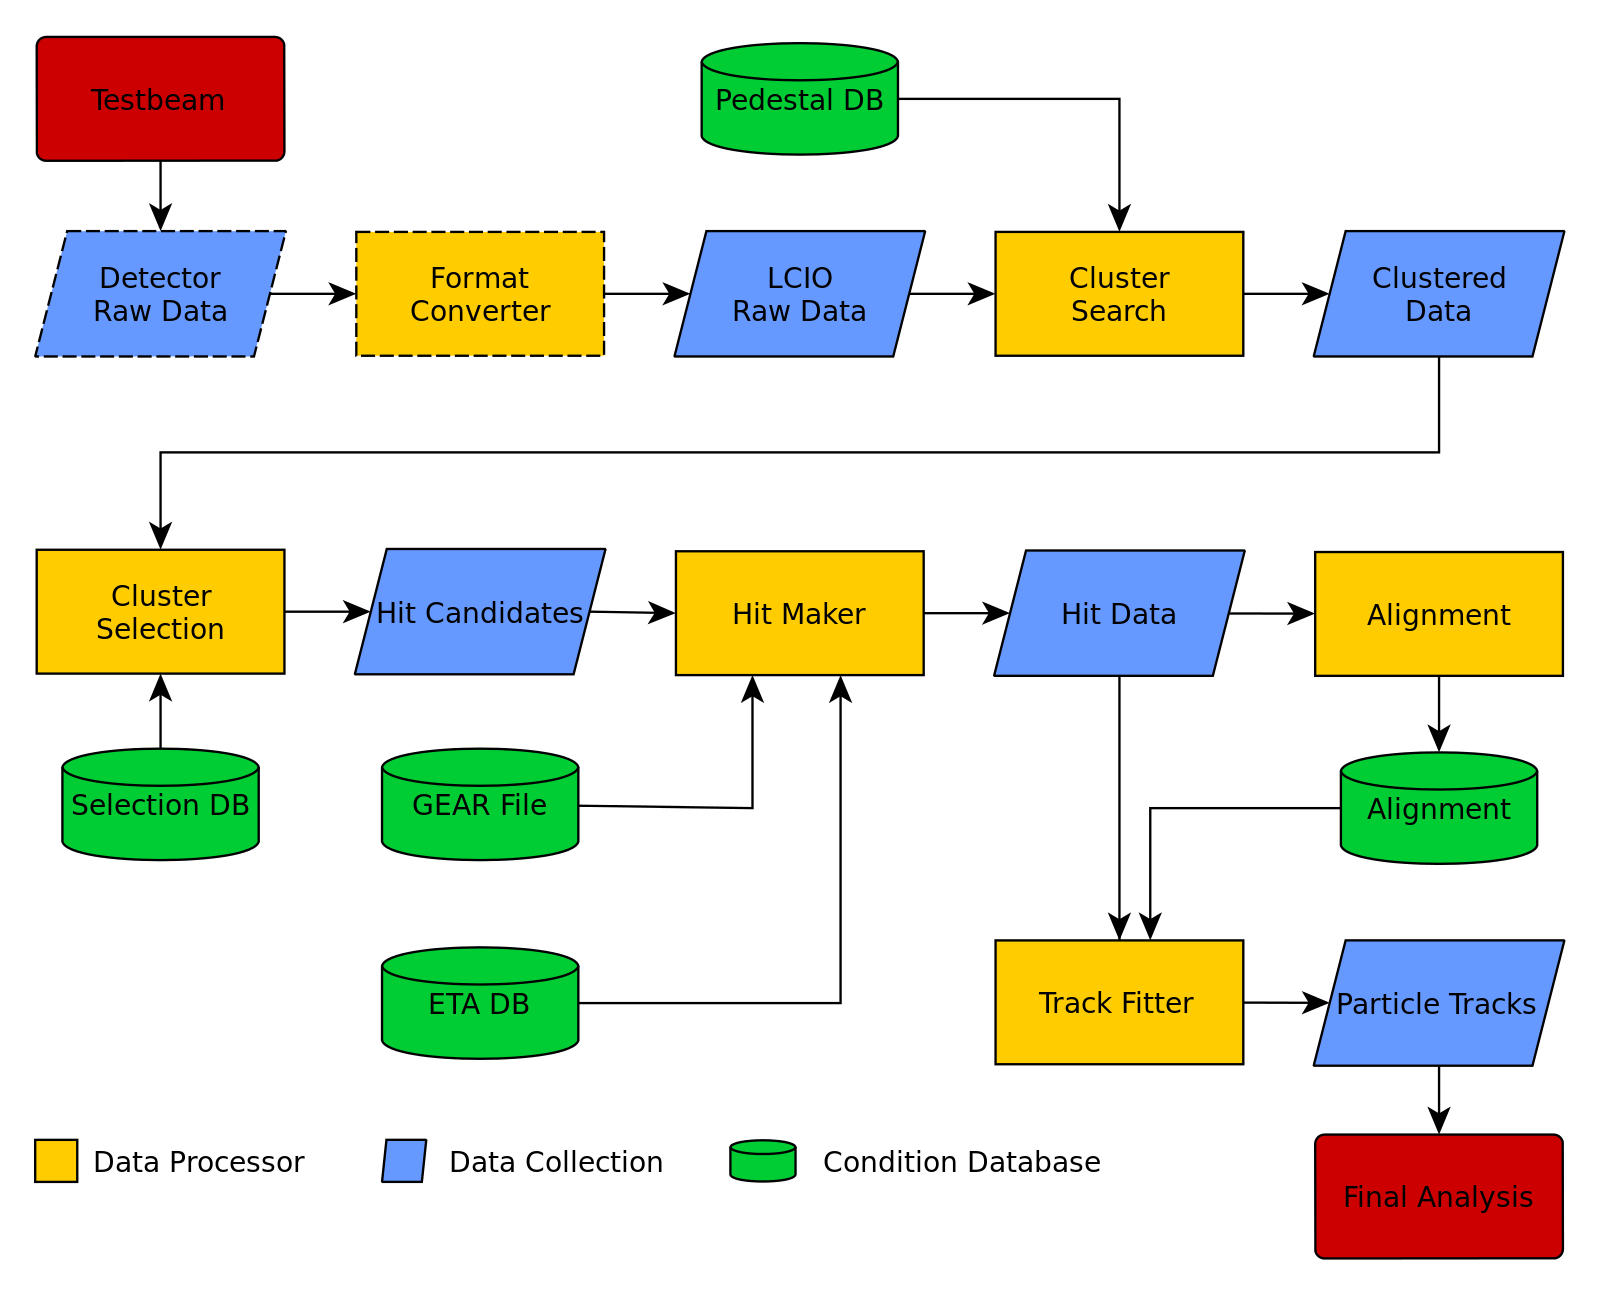
\includegraphics[scale=0.3]{eutel-strategy.png}
	\caption{\textit{The EUTelescope framework}}
\end{figure}
\subsection{Software}
\subsubsection{LCIO}
\paragraph{}
Data in EUTelescope is stored in the Linear Collider Input Ouput (LCIO) data format. LCIO is an event-based data format and persistence framework that is widely used for linear collider studies and reconstruction within the HEP community. A test beam experiment, with a EUDET style telescope, is essentially a linear collider experiment, so this data format lends itself well to EUTelescope. The details of LCIO are covered by this guide in section 1.3.1 and the online documentation and can be located here: \url{http://lcio.desy.de}.
\subsubsection{ILCSoft[7]}
\paragraph{}
ILCSoft is the name given to a suite of software packages that were created to enable the design and analysis of the future International Linear Collider (ILC). Currently the ILCSoft suite includes the following software: (The packages that are used by EUTelescope, and are hence relevant to this guide, are emboldened with a short description provided.) 
\begin{itemize}
\item Brahms
\item CED
\item Overlay
\item CEDViewer
\item \textbf{Gear} - A geometry description toolkit.
\item \textbf{EUTelescope} - A group of Marlin processors to reconstruct EUDET style telescope data.
\item LCCD
\item \textbf{LCIO} - A data format and persistence framework. 
\item LCFIVertex
\item ilcinstall
\item \textbf{Marlin} - Modular application frame work for linear collider reconstruction and analysis. The framework is based on the LCIO format.
\item MarlinReco
\item MarlinTPC
\item MarlinUtil
\item Mokka
\item \textbf{RAIDA} - An Abstract Interfaces for Data Analysis (AIDA) implementation based in ROOT, to allow for the direct filling of ROOT objects from AIDA.
\end{itemize}
\subsubsection{Marlin[8]}
\paragraph{}
Marlin (Modular Analysis and Reconstruction for the LINear collider) is an LCIO based modular application framework. Marlin does the actual processing and execution of jobs submitted to EUTelescope, and as such, in this sense it is the backbone of EUTelescope. Marlin will read in \textit{.slcio} data files, as well as steering files (see section 3.2.2) to do determine which processors are invoked, and therefor how the data is processed.
\paragraph{}
For further information, see the Marlin documentation: \url{http://ilcsoft.desy.de/Marlin/current/doc/html/index.html}.
\subsubsection{The RAIDA Processor[2]}
\paragraph{}
Another framework embedded in the ILCsoft suite is the Abstract Interface for Data Analysis (AIDA). AIDA provides common interfaces in either C ++ or Java for different data analysis tools and tries to unify the communication with these tools. The implementation used in the EUTelescope package and therefore in this beam test analysis is the ROOT implementation of AIDA, called RAIDA. The main objective of RAIDA is to provide access to ROOT objects within the ILCsoft environment and allow their creation.
\paragraph{}
Usually the RAIDA processor instance is called as the first Marlin processor directly after loading the LCIO file which will be processed. Once per run the AIDA histograms of each processor using the interface are initialized. During the event processing stage information is added to the histograms. After the run has finished all histograms are written to a ROOT file and are accessible through the ROOT interface. Almost every EUTelescope processor implements a RAIDA instance to write status histograms for the current analysis step. The EUTelFitTuple uses RAIDA to write the created particle tracks and hit measurements to a ROOT tree to allow an easy inspection of all events. Usually a boolean parameter like the HistogramSwitch is provided within every processor to turn the histogram creation on or off.
\subsection{File Formats}
\subsubsection{LCIO Data Format[3]}
\paragraph{}
The data format used in the ILCsoft package is the Linear Collider I/O (LCIO) persistency framework and event data model. It provides user interfaces in different programming languages (C ++, Java, Fortran) and is designed to cover all fields of detector research and development. Especially the gap between detector simulation and reconstruction should be closed with a unique data format for both sides.
\paragraph{}
The interface provided by the library is abstract and hides the actual storing mechanisms from the user. This allows an easy integration into other projects without having to deal with the underlying data model and prevents the user from non-trivial code changes in case the model is altered. This is of special importance since the ILC projects are still under heavy development and implementations are likely to change.
\paragraph{}
LCIO is an event-based data format. All data belonging to one trigger decision and detector readout is stored together and can be accessed via the corresponding event number. An event consists of the event header and the actual data. The header contains information on the detector, the timestamp, and the run number. The event data is stored in collections of different types. Each type is specific for a certain stage of the pattern recognition chain. While the TrackerRawData (full-frame data) and TrackerData (zero-suppressed data) contain raw detector data, the TrackerPulse collections are used to store the processed clusters. After the track reconstruction procedure thehits and tracks are stored in TrackerHit and Track collections, respectively. Each collection contains specific data entities which are all labeled with a unique hexadecimal ID. These IDs connect the otherwise independent collections and allow easy cross-references, e.g. referencing all pixel hits belonging to a particular cluster. This way a reconstructed track can still contain all information down to the original raw detector data.
\paragraph{}
Two command line tools are particularly useful for fast inspection of LCIO file contents. The structure and included collections can be obtained using the anajob command. The content of these collections in a single event can be extracted from the LCIO file using the dumpevent command. In this output the correlation of the different data entities can be observed by comparing the corr.Data fields and the entity IDs.
\subsubsection{GEAR - Telescope Geometry Description[4]}
\paragraph{}
On the software side the different telescope geometries are implemented using the Geometry API for Reconstruction (GEAR) markup language. GEAR is a geometry description toolkit which is part of the ILC reconstruction software. It implements an abstract interface for the layout description of detectors for event reconstruction. The geometry described in a GEAR file is simplified and therefore cannot be used for a detailed Monte Carlo simulation of the detector. For reconstruction on the other hand only a few parameters are enough since no precise material allocation information is needed to calculate the particle behavior.
\paragraph{}
The integration into the EUTelescope framework allows the usage of the unchanged processor chain with the same parameters for different detector geometries, switching between them just by loading another GEAR file. The processors within the chain obtain all information needed for their algorithm directly from the GEAR framework, e.g. the pixel pitches and plane distances for the coordinate transformation from local on-plane coordinates to the global telescope frame of reference.
\paragraph{}
GEAR uses XML markups for the detector description, whereof several packages for different purposes are provided. In case of silicon pixel detectors the GearType SiPlanesParameters can be used providing all properties needed to describe a tracking telescope. The XML markup contains a hierarchical description of the detector parts starting with the whole detector as well as global parameters such as magnetic field. The telescope can be divided into layers. Every layer represents one particular telescope plane in the GEAR description. This allows e.g. the usage of several sensor types with different properties such as pixel pitch or sensor thickness in different telescope planes which is especially interesting for telescopes with exchangeable DUT. A layer consists of a ladder and a sensitive part. These elements hold the basic parameters such as position, rotation, size, pitch, and the radiation length of the sensitive detector material. Rotations of telescope planes can be obtained either by using a simple 2 × 2 rotation matrix for the $xy$ plane or the Euler angles for 3-dimensional rotations.
\section{Installation[5]}
\paragraph{}
Since EUTelescope uses parts of the ILCsoft package it is convenient to use the ILCsoft installation scripts to put everything in place. EUTelescope only uses a small subset of the tools provided by ILCsoft and we prepared some ILCsoft Installer configuration to reduce the amount of data and the time to build the packages. This configuration comprises everything you should normally need to run telescope analysis jobs. However, if you have special demands and need additional packages or want e.g. 3D event data viewer capabilities you might have to reconfigure and rebuild yourself.
\paragraph{Please note...}
It is recommended that you install EUTelescope in a directory where you have \textit{sudo} rights. Many errors occur during the installation due to not having the correct libraries, as well as other issues that require elevated permissions to correct. Installing EUTelescope in a directory where you have elevated permissions will make your life easier. If it is not possible to install this with elevated permissions, the Ubuntu Software Center provides a means of acquiring a lot of the required libraries, without the need for \textit{sudo}. Unfortunately not all the libraries will be found this way, use of the software center will reduce the number of requests you have to make to your system administrator!
\subsection{System Requirements}
\paragraph{}
EUTelescope (or rather Marlin, the event processor provided by ILCsoft) is GRID capable so you can either run your analysis using GRID computing or just locally on your machine or workgroup server. Installing the standalone version of EUTelescope and the ILCsoft framework in the minimal configuration provided here requires only about 1.5 GB disk space. However, if you decide to perform a full setup with all packages provided by ILCsoft the \textbf{installation requires about 4GB disk space}.
\paragraph{}
It is highly recommended to have \textbf{more than 2 GB RAM} available for running EUTelescope analysis and to use a 64bit kernel to make use of the available RAM.
\subsection{Support Operating Systems and Architectures}
\paragraph{}
The following Linux distributions are currently supported and tested to work well with EUTelescope and the installation procedures described here:\\
\begin{itemize}
	\item Scientific Linux 5.8 (Boron), x86\_64 (64bit), i386 (32bit)
	\item Ubuntu 12.04 LTS (Precise), x86\_64 (64bit), i386 (32bit)
\end{itemize}
\paragraph{}
We highly recommend to use the 64bit versions to allow EUTelescope to make best use of the available RAM. Minor updates of these systems (such as Ubuntu 12.04.1 or Scientific Linux 5.9) should run smoothly. Other distributions have been reported to work (e.g. Ubuntu up to 13.04 and Scientific Linux 6.4) but have not been as thoroughly tested.
\subsection{Standalone Installation}
\paragraph{}
The standalone installation procedure will download and compile the sources of EUTelescope and selected ILCsoft packages required for running EUTelescope. On a modern machine, this should take between 30 - 60 minutes.
\subsubsection{Prerequisites I: packet installation}
\paragraph{}
First, you need to install all packages required for the compilation of the ILCsoft packages and of EUTelescope. These differ slightly between the distributions:\\
\paragraph{Scientific Linux 5.8 (Boron)}
\begin{minted}[breaklines]{bash}
su -c "yum install gcc-c++ gcc-gfortran subversion java-1.7.0-openjdk-devel gsl-devel libX11-devel \
      libXpm-devel libXft-devel libXext-devel gcc44-gfortran python-devel"
\end{minted}
\paragraph{Ubuntu 12.04 LTS (Precise)}
\begin{minted}[breaklines]{bash}
sudo apt-get install build-essential gfortran cmake subversion default-jdk libgsl0-dev libxpm-dev \
      libxft-dev libx11-dev libxext-dev python-dev
\end{minted}
Please note: It is very important that you use at least version 4.8 of the GCC compiler suite. This is to ensure that source code files containing C++ 11 features can be compiled correctly. If using Scientific Linux, these compilers are available as part of the SCL software collections framework. Please read about them here: \url{http://linux.web.cern.ch/linux/devtoolset/}.
\paragraph{}
Once you have installed the developer toolset packages (these are already installed if you are a NAF user) they are very easy to activate. Do so with the following command:
\begin{minted}[breaklines]{bash}
scl enable devtoolset2 bash
\end{minted}
This will set your GCC suite to version 4.8 as required. Do not use devtoolset1.1 as it is not sufficient; devtoolset2, 3 and 4 are all fine to use.
\subsubsection{Prerequisites II: prepare installation path and download installer}
\paragraph{}
Prepare the ILCsoft environment by specifying and creating the desired installation path:\\
\begin{minted}[breaklines]{bash}
export ILCSOFT=/path/where/you/want/to/install
\end{minted}
\begin{minted}[breaklines]{bash}
mkdir -p $ILCSOFT
\end{minted}
\paragraph{}
Now the latest version of the ILCsoft Installer can be checked out from the Subversion repository using:\\
\begin{minted}[breaklines]{bash}
cd $ILCSOFT
\end{minted}
\begin{minted}[breaklines]{bash}
svn co https://svnsrv.desy.de/public/ilctools/ilcinstall/tags/v01-17-03-eutel ilcinstall_v01-17-03-eutel
\end{minted}
\paragraph{}
To use git version follow:\\
\begin{minted}[breaklines]{bash}
cd $ILCSOFT
\end{minted}
\begin{minted}[breaklines]{bash}
svn co https://svnsrv.desy.de/public/ilctools/ilcinstall/branches/eutel-git ilcinstall_eutel-git
\end{minted}
\paragraph{Prerequisites III: Check the version of EUTelescope (and EUDAQ) to be installed}
Before starting the installation, please check that the file\\
\begin{minted}[breaklines]{bash}
$ILCSOFT/ilcinstall_v01-17-03-eutel/releases/v01-17/release-versions.py
\end{minted}
\paragraph{}
or for git version\\
\begin{minted}[breaklines]{bash}
$ILCSOFT/ilcinstall_eutel-git/releases/v01-17-05/release-versions.py
\end{minted}
sets the version numbers of EUTelescope and EUDAQ that you wish to install (set by the variables Eutelescope\_version and Eudaq\_version respectively). Valid values for EUTelescope are for example ``v00-09-02'' for the 0.9.2 release, or ``HEAD'' for the development branch (i.e. the SVN trunk). For EUDAQ (which is used for the data conversion into LCIO) you need to supply the SVN path, e.g. ``tags/v01-00-00'' for the 1.0 release or ``trunk'' for the development version.
\paragraph{Run the installation}
For SVN version:\\
\begin{minted}[breaklines]{bash}
cd $ILCSOFT/ilcinstall_v01-17-03-eutel
\end{minted}
\begin{minted}[breaklines]{bash}
./ilcsoft-install -i examples/eutelescope/release-standalone.cfg
\end{minted}
For git version:\\
\begin{minted}[breaklines]{bash}
cd $ILCSOFT/ilcinstall_eutel-git
\end{minted}
\begin{minted}[breaklines]{bash}
./ilcsoft-install -i examples/eutelescope/release-standalone.cfg
\end{minted}
\paragraph{}
Now is a good time to grab a coffee! When you are back, EUTelescope should be ready to run, as soon as you set up your environment correctly (see Operation).
\paragraph{}
Please note: The ROOT installation files location has moved and it is not clear if the install scripts have been updated to reflect this. Before running your installation, open up the file "\$ILCSOFT/ilcinstall\_eutel-git/ilcsoft/root.py" with a text editor. Change the old self.download.url ROOT link to ``self.download.url ='https://root.cern.ch/download/root\_v\%s.source.tar.gz' \% self.version''. This will ensure that ROOT downloads correctly. 
\subsection{Alternative installation (for ITk strips users)}
\paragraph{}
The following section details an alternative installation procedure that is used by the ATLAS ITk strips group. This alternative installation is required in order to ensure that the strips user has all of the required files, for tasks like pattern recognition, and that the correct version of GBL and EUDAQ are used. Please note that this installation has been trialed for systems running Scientific Linux only. Ubuntu installs via this method are untested, but may work. If you are not a Scientific Linux user, please consider using one of the VirtualBox Virtual Machines (VMs) that have been set up for EUTel\_Strips users. They are an out-of-the-box solution
\paragraph{Step 1}
Follow all the standard installation instructions to the end (detailed in section 2 of this guide). Make sure that you are using at least version 4.8 of the GCC compiler suite; this is because C++ 11 features are used in the code, and earlier compilers are not compatible with this. Do not use package managers like Linuxbrew to install the compilers. Whilst they appear to offer an easy option for getting the compilers one needs, they do not work for this installation as they are not picked up by the install scripts.
\paragraph{Step 2 - EUTelescope repository checkout}
This steps requires the cloning of a repository owned by Alex Morton. Initially you must navigate to the \$EUTELESCOPE folder. Once there run the following commands:
\begin{minted}[breaklines]{bash}
git remote add alexRep https://github.com/AlexanderMorton/eutelescope.git
git pull alexRep
git checkout alexRep/X0 -b alexRep_X0_local
\end{minted}
These commands add a remote, pull it down to the local machine, and then create a local branch for the user to work with.
\paragraph{Step 3 - EUDAQ checkout}
Navigate to:
\begin{minted}[breaklines]{bash}
$EUTELESCOPE/external/eudaq
\end{minted}
Now run the following commands:
\begin{minted}[breaklines]{bash}
git clone https://github.com/eudaq/eudaq.git v1.4.5
cd v1.4.5
git tag -l  	//To view what tags are available
git checkout tags/v1.4.5
git checkout -b v1.4.5_local
\end{minted}
This checks out one of the required version of EUDAQ and creates a local branch for the user.
\paragraph{}
Note that sometimes the version you want to checkout won't be a tag, but a branch. This is the case for EUDAQ v1.7-dev. When you are checking out a branch from a remote you can do it in the following way:
\begin{minted}[breaklines]{bash}
git branch -r //This will show the branches that are available on the remote
git checkout -b local_branch_name origin/branch_name
\end{minted}
\paragraph{}
So in the case of v1.7-dev, you can type:
\begin{minted}[breaklines]{bash}
git checkout -b v1.7-dev origin/v1.7-dev
\end{minted}
\paragraph{}
This will create the local branch \textit{v1.7-dev} and then checkout the remote branch called \textit{v1.7-dev}, and merge it into the local branch. This will have the same effect the checkout using tags, so now you have two methods to check out specific versions from the EUDAQ git repository.
\paragraph{Step 4 - Building EUDAQ}
To build this version of EUDAQ you must use at least CMake 3.5.2. This is fairly easy to install yourself from the CMake website. Just download the tarball and follow the instructions, which mostly consist of running an install script.
\paragraph{}
Continuing from step 3, change directory into the build directory:
\begin{minted}[breaklines]{bash}
cd build
\end{minted}
Now make sure you are using at least GCC version 4.8, enable this by typing:
\begin{minted}[breaklines]{bash}
scl enable devtoolset2 bash
\end{minted}
into your terminal; see section 2.3.1 if you are not aware of the devtoolset collection. If you don't wish to use the developer tool sets then ensure you have the correct compiler by another means. Also, make sure you are aware of where the compilers are installed: you will need this shortly. Compilers that are part of devtoolset2 are stored in the following location:
\begin{minted}[breaklines]{bash}
/opt/rh/devtoolset-2/root/usr/bin
\end{minted}
Now, from the build directory, start the building process. Before doing this it is recommended that you setup an environment variable that contains the path to your GCC suite. This is because certain options are needed to be passed to CMake and this will reduce the typing necessary. Do the following:
\begin{minted}[breaklines]{bash}
export COMPILER_LOC=/opt/rh/devtoolset-2/root/usr/bin
\end{minted}
Make sure you use the correct path for your compiler. Once the variable is set up, run the following command from the build directory:
\begin{minted}[breaklines]{bash}
/path/to/your/CMake/v3.5.2/installation/bin/cmake -DCMAKE_CXX_COMPILER=$COMPILER_LOC/g++ -DCMAKE_CC_COMPILER=$COMPILER_LOC/gcc ..
\end{minted}
This command ensure that you use the CMake version needed as well as forcing the system to build using the compilers you want, if you leave the options out then you will find that some part of the install script specifies the use of GCC v4.4 and as such your build will fail. Once the project has built, type:
\begin{minted}[breaklines]{bash}
make install
\end{minted}
to install the project.
\paragraph{}
Now that the install is complete, you must rebuild and reinstall using some additional CMake options. Run the following from the build directory:
\begin{minted}[breaklines]{bash}
/path/to/your/CMake/v3.5.2/installation/bin/cmake -DCMAKE_CXX_COMPILER=$COMPILER_LOC/g++ -DCMAKE_CC_COMPILER=$COMPILER_LOC/gcc -DUSE_LCIO=ON -DBUILD_nreader=ON ..

make install
\end{minted}
Once this step has successfully completed, you can move onto step 5.
\paragraph{Step 5 - Building EUDAQ v1.6.0 and v1.7-dev}
For step 5 you simply repeat step 4 exactly, replacing any reference of v1.4.5 of EUDAQ with v1.6.0, and then again for EUDAQ v1.7-dev, bearing in mind that v1.7-dev is not a tag, but a branch, so you must use the branch checkout method detailed in \textit{step 3}. 
\paragraph{}
Once this is complete you must update the build\_env.sh script so that it uses the correct EUDAQ version. To do this open
\begin{minted}[breaklines]{bash}
$EUTELESCOPE/build_env.sh
\end{minted}
in your preferred text editor and make the changes. Searching for EUDAQ in the editor should reveal 3 locations that need updating. Once this is finished, you're all set!
\subsection{Installation for Fedora systems}
\paragraph{}
The following commands can be followed to install a EUTelescope on Fedora systems. The guide assumes that the Fedora system is brand new and so installs all the prerequisites that are required. If the Fedora system is not brand new this is not a problem, just follow the instructions as normal.
\paragraph{}
Open up a new terminal and type the following: Please note that certain commands require elevated permissions depending on your setup and so you may have to re-run certain commands with ``sudo''.
\begin{minted}[breaklines]{bash}
export ILCSOFT=/ilcsoft
\end{minted}
This sets the top-level ILCsoft directory.
\begin{minted}[breaklines]{bash}
dnf -y install wget automake
\end{minted}
Note, commands invoking the \textit{dnf} package manager are likely to need ``sudo''.
\begin{minted}[breaklines]{bash}
wget ftp://rpmfind.net/linux/fedora/linux/releases/23/
Everything/x86_64/os/Packages/g/gsl-devel-1.16-17.fc23.x86_64.rpm
\end{minted}
\begin{minted}[breaklines]{bash}
wget ftp://rpmfind.net/linux/fedora/linux/releases/23/
Everything/x86_64/os/Packages/g/gsl-1.16-17.fc23.x86_64.rpm
\end{minted}
Please note: the only ``space'' character in the above commands is between the ``wget'' and the URL. Enter the URL as a single line with no breaks or spaces. 
\begin{minted}[breaklines]{bash}
rpm -U gsl-1.16-17.fc23.x86_64.rpm

rpm -U gsl-devel-1.16-17.fc23.x86_64.rpm
\end{minted}
Now to install the remaining prerequisite software:
\begin{minted}[breaklines]{bash}
dnf -y install gcc-c++ gcc-gfortran subversion java-1.8.0-openjdk-devel libX11-devel libXpm-devel libXft-devel libXext-devel python-devel tar make cmake which git
\end{minted}
\paragraph{}
Now that the prerequisites are in place it is time to get the source files and do the install.
\begin{minted}[breaklines]{bash}
mkdir -p $ILCSOFT
\end{minted}
\begin{minted}[breaklines]{bash}
svn co https://svnsrv.desy.de/public/ilctools/ilcinstall/branches/v01-17-10-eutel-dev/ $ILCSOFT/ilcinstall_v01-17-10-eutel
\end{minted}
\begin{minted}[breaklines]{bash}
$ILCSOFT/ilcinstall_v01-17-10-eutel/ilcsoft-install -i -v $ILCSOFT/ilcinstall_v01-17-10-eutel/examples/eutelescope/release-standalone.cfg
\end{minted}
\section{Operation}
\subsection{Setting the EUTelescope Environment[5]}
\paragraph{}
Before any attempt to use ILCsoft and EUTelescope in a meaningful way you must load the environment variables:\\
\begin{minted}[breaklines]{bash}
cd $ILCSOFT/Eutelescope/v00-YY-XX/
\end{minted}
\begin{minted}[breaklines]{bash}
.source build_env.sh
\end{minted}
where the ``YY-XX'' needs to be replaced with the actual version of EUTelescope you've installed.
\paragraph{}
If you are running csh or tcsh Shell you should source a ``build\_env.csh''. The script initializes the \textit{PATH} and \textit{LD\_LIBRARY\_PATH} variables. A \$EUTELESCOPE variable is also introduced here. Echoing \$EUTELESCOPE is a good way to check if your build environment has loaded correctly. If it hasn't then the variable will not be set.
\paragraph{}
It is recommended to create a symlink between the \textit{EUTelescope} install location and your home directory for quick access.\\ 
Do this by running: 
\begin{minted}[breaklines]{bash}
cd ~
ln -s <folder/you/want/to/link/to> <name of symlink folder>
\end{minted}
This will create a folder in the home directory with the name specified. So for example the command should look something like this:
\begin{minted}[breaklines]{bash}
cd ~
ln -s /nfs/dust/atlas/user/daubneyt/ilcsoft/v01-17-05/Eutelescope/trunk EUTelescope
\end{minted}
\subsection{Processors}
\paragraph{}
This can be a list of processors that are available.
\subsection{Steering files[6]}
\paragraph{}
The steering files control which processors, with which set of options, are executed when passing the file to Marlin. The steering files are written in the XML markup format.
\paragraph{}
As a starting point, EUTelescope provides sets of steering files as examples, where every steering file corresponds to a step in the analysis chain. These examples can be found in the \textit{jobsub/examples} folder - please note the accompanying README files.
\paragraph{}
Whether you use an example as basis for your own analysis and you would like to add a missing processor, or whether you create the steering templates from scratch, ILCSoft offers tools that make these task significantly easier! The following steps show how you can create a new steering template from scratch for job submission with \textit{jobsub} (discussed later), using Marlin. 
\paragraph{How to generate an example steering file}
Provided that the EUTelescope environment has been built, one can type the following into the terminal to produce and example steering file. This file will show the user how the steering file should be structured, and exactly what processors are available.
\begin{minted}[breaklines]{bash}
Marlin -x > example.xml
\end{minted}
This produces the example steering file and writes it to the current working directory. This can then be opened for inspection with Vim, or any other text editor, or IDE, available.
\paragraph{}
This example steering file can be used as the basis to the steering files that will be required when executing steps in the reconstruction chain.
\paragraph{Creating a steering file from the example file}
First, copy the XML structure including the \textit{\textless marlin\textgreater}, \textit{\textless execute\textgreater} and \textit{\textless global\textgreater} sections (including closing tags in the end of the file!) into a new XML file that you will use as the steering file for the given analysis step.
\paragraph{}
Next, copy the \textit{\textless processor\textgreater} section of every processor you would like to execute in your analysis and adjust its options according to your needs. Any option that varies from run to run (e.g. the file name, beam energy, thresholds, ...) should be filled with a placeholder variable that can be substituted by \textit{jobsub}. This placeholder can have any name (capitalization is ignored) but must be enclosed in '@' signs. Make sure that you use the placeholder @RunNumber@ for every place where you want the run number to appear as this is the only variable required by \textit{jobsub}. Make sure that all processors are also included in the \textit{\textless execute\textgreater} section, or they will not be run by Marlin!
\paragraph{}
Once this is complete, the XML file will now be ready to serve as a steering file for Marlin, for the given reconstruction step.
\subsection{Job submission with \textit{jobsub}[9]}
\paragraph{}
As previously mentioned, the execution of EUTelescope code is via the invocation of Marlin (see section 1.2.3), and therefore it is driven by steering files, as well as config files and run lists (discussed later). In order to submit these jobs for Marlin processing, a python tool, called \textit{jobsub}, is used. This has the effect of making the specific analysis chain that a user wishes to run, much easier to control.
\subsubsection{Usage and list of available \textit{jobsub} arguments}
\paragraph{}
The user can invoke \textit{jobsub} in the following way, from the terminal:
\begin{minted}[breaklines]{bash}
jobsub [-h] [--option NAME=VALUE] [-c FILE] [-csv FILE] [--log-file FILE] [-l LEVEL] [-s] [--dry-run] jobtask [run [runs ...]]
\end{minted}
\paragraph{}
Below you will find a table that describes the type and usage of all the options that are available when submitting jobs with \textit{jobsub}.
\pagebreak
\begin{table}[!ht]
\centering
\caption{Table detailing the possible options that can be used with \textit{jobsub}.}
\label{jobsub_options}
\begin{tabular}{|p{0.2\linewidth}|p{0.2\linewidth}|p{0.4\linewidth}|p{0.2\linewidth}|}
\hline 
\textbf{Argument}                        & \textbf{Argument type} & \textbf{Description}                                                                                                                                                                                                                                       & \textbf{Example values}        \\ \hline
jobtask                                  & positional             & Details the task (or processor) that the user wishes to execute. The task names are user specified and arbitrary.                                                                                                                                          & convert, hitmaker, align, etc. \\ \hline
runs                                     & positional             & Lists the runs that are to be analysed. The runs can be specified as a single value or a range of values.                                                                                                                                                  & 1001, 1002-1005.               \\ \hline
-h, --help                               & optional               & Shows the help menu and then quits Marlin.                                                                                                                                                                                                                 & N/A                            \\ \hline
-o NAME=VALUE, --option NAME=VALUE       & optional               & This switch allows the user to specify further options. It can be specified multiple times or it also accepts a comma separated list of options. Any options that get specified using this switch will overwrite any config file options of the same name. & beamenergy=5.3                 \\ \hline
-c FILE, --conf-file FILE, --config FILE & optional               & Load the config file specified with FILE.                                                                                                                                                                                                                  & Any valid config file name.    \\ \hline
--concatenate                            & optional               & Concatenate all runs into first run by combining every option that includes the string @RunRance@ multiple times, once for each run of the range specified.                                                                                                & N/A                            \\ \hline
-csv FILE, --csv-file FILE               & optional               & Load additional run-specific variables from table in a CSV format.                                                                                                                                                                                         & Any valid CSV file name.       \\ \hline
--log-file FILE                          & optional               & Specifies the file to save the submission log to.                                                                                                                                                                                                          & Any valid log file name.       \\ \hline
-l LEVEL, --log LEVEL                    & optional               & Defines the verbosity level used in the log file.                                                                                                                                                                                                          & debug, info, warning, error.   \\ \hline
-s, --silent                             & optional               & Suppress non-error Marlin output to the terminal.                                                                                                                                                                                                          & N/A                            \\ \hline
--dry-run                                & optional               & Write steering files but suppress the actual execution of Marlin.                                                                                                                                                                                          & N/A                            \\ \hline
\end{tabular}
\end{table}
\subsubsection{Steering files and \textit{jobsub}}
\paragraph{}
Steering file templates are valid Marlin steering files where specific values are replaced by variables in the form \textit{@VariableName@}. When invoking \textit{jobsub} these placeholders get filled with a user-defined value that can be specified in the following way (in order of precedence): command-line arguments, config files or a table with a row for each number processed. There is one predefined placeholder, called @RunNumber@, which will be substituted with the current run number (padded with leading zeros up to 6 digits e.g. 001234).
\subsubsection{\textit{jobsub} configuration - config files}
\paragraph{}
Config files are created to help pass variable values efficiently into EUTelescope, as well as specify important parameters like file paths. \textit{Table 1} describes how you can specify the config file you wish to use when invoking \textit{jobsub}.
\paragraph{}
In the context of the \textit{EUTelescope} framework, config files are human readable text files that are split up into sections, denoted by \textit{[SECTION NAME]}. In every config file there is a \textit{[DEFAULT]} section, labeled exactly as shown, and then there are a series of task specific sections that will vary depending on the users intentions for their analysis.
\paragraph{Key things to note about config files} The key features of config files are described in the list below:
\begin{itemize}
\item Interpolation of format strings is supported.
\item Some default interpolations are \textit{\%(home)s} and \textit{\%(eutelescopePath)s} which are setup with the environment variables.
\item Comments are prefixed with \textit{\#} or \textit{;}.
\item The "@RunNumber@" string will be replaced in the template file after all other variable strings are filled. This means that you can use the \textit{@RunNumber@} placeholder inside options, such as the file name.
\end{itemize}
\paragraph{}
The best way to understand the config files and their structure is to look at the files themselves. A good starting point is the config file in the datura-noDUT example, which can be found here:
\begin{minted}[breaklines]{bash}
jobsub/examples/datura-noDUT/config.cfg
\end{minted} 
More information on can be found here: \url{http://docs.python.org/2/library/configparser.html}
\subsubsection{\textit{jobsub} configuration - tables}
\paragraph{}
Another option available to the user for the configuration of \textit{EUTelescope} is the use of tables. These tables are formatted in a specific way as described below and are saved in a CSV text file format.
\paragraph{Key points for the creation of tables}
\begin{itemize}
\item File format: \textbf{either} export from LibreOffice with default settings (UTF-8, comma-separated, text-field delimiter: ") \textbf{or} use and emacs org-mode table (\url{http://orgmode.org/manual/Tables.html}).
\item Commented lines are denoted with a \textit{\#} prefix.
\item First row of the table must supply the column headers which determine the variables to be replaced and one of the columns in the table must be labeled ``RunNumber''. (This is not case sensitive.)
\item Values in the table are only read in for variables that have not been filled by the command line options, or the config file. Tables have the lowest priority.
\end{itemize}
\paragraph{}
The image below shows how a simple emacs org-mode table appears. With the following table, the variable \textit{@BeamEnergy@} will get replaced when the corresponding run is being processed.
\begin{figure}[!ht]
	\centering
	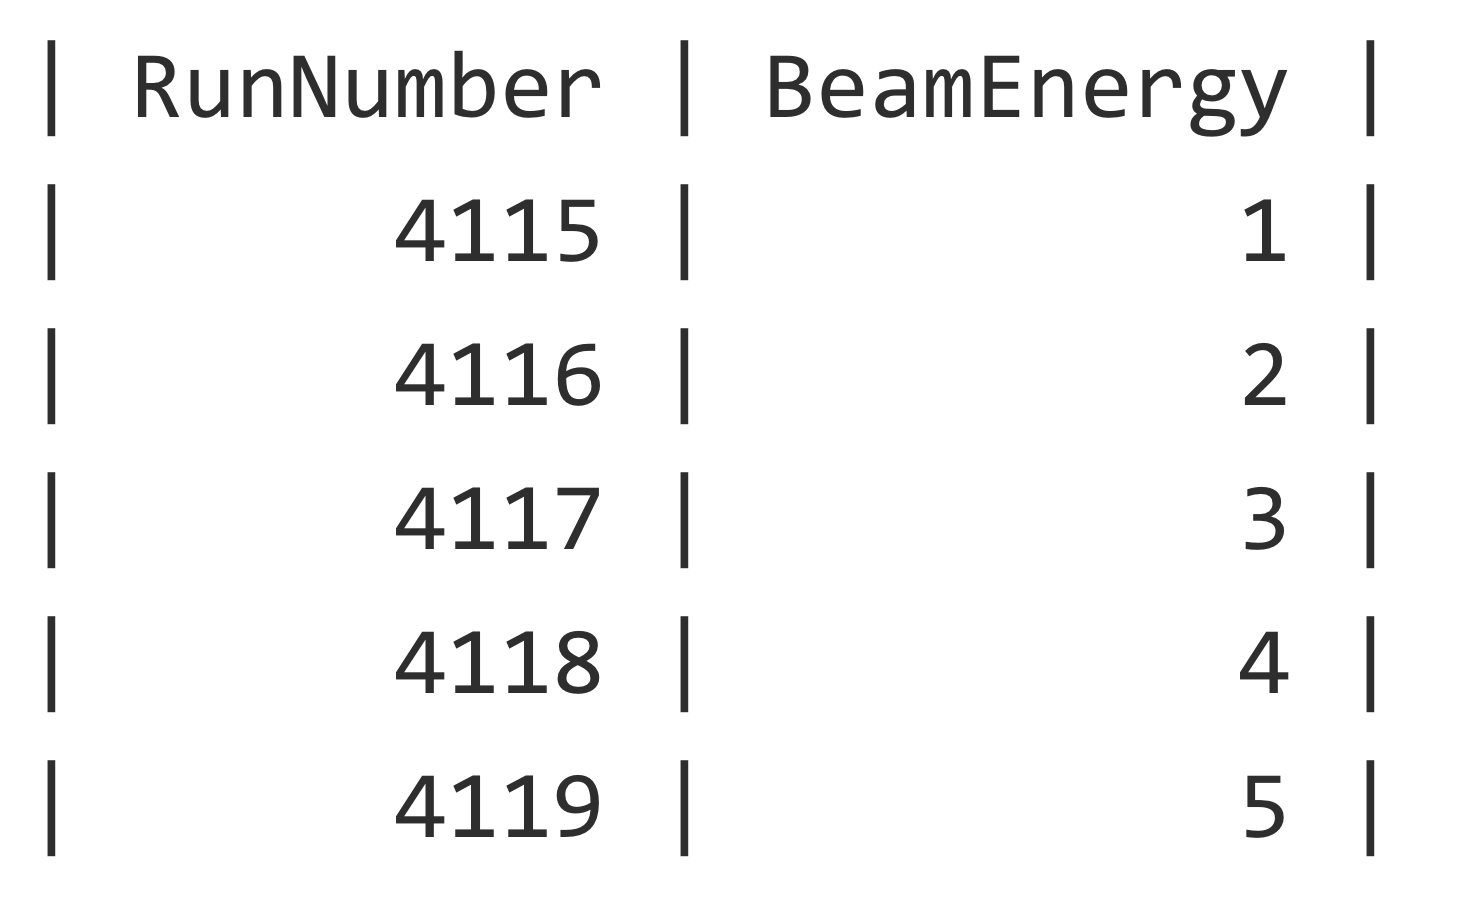
\includegraphics[scale=0.25]{orgtable.png}
	\caption{\textit{A simple org-mode table.}}
\end{figure}
\subsubsection{\textit{jobsub} configuration - concatenation}
\paragraph{}
If you have an option e.g. the LCIO input files that you want to fill with several runs in one steering file, you can use a command line switch to activate concatenation. This replaces any steering file placeholder, whose corresponding option contains the string "@RunRange", multiple times, once for every run specified.
\paragraph{}
The following command:
\begin{minted}[breaklines]{bash}
jobsub --concatenate --option LCIOInputFiles=/my/path/to/data/@RunRange.lcio align 1234 1235-1237
\end{minted}
\paragraph{}
will create only one steering file, for run 1234, where the place holder \textit{@LCIOInputFiles@} is replaced by its value 4 times and \textit{@RunRange@} is replace by values from 1234 to 1237.
\paragraph{}
This is to say that (in the template file):
\begin{minted}[breaklines]{bash}
<parameter name="FileName" type="string" value= @LCIOInputFiles@/>
\end{minted}
\paragraph{}
becomes:
\begin{minted}[breaklines]{bash}
<parameter name="FileName" type="string" value= /my/path/to/data/1234.lcio 
        /my/path/to/data/1235.lcio /my/path/to/data/1236.lcio /my/path/to/data/1237.lcio/>
\end{minted}
\paragraph{}
Concatenation used in this way has potential uses in scenarios where the user may want to combine several runs to perform an alignment step.
\subsection{Dumpevent}
\paragraph{}
Dumpevent is a simple tool that allows the user to inspect the contents of their \textit{.slcio} files. This is very useful for both learning how to use \textit{EUTelescope} as well as finding any potential issues that may arise during the course of the analysis.
\paragraph{Usage of Dumpevent}
In order to invoke Dumpevent, use the following command:
\begin{minted}[breaklines]{bash}
dumpevent my_file.slcio <event_number>
\end{minted}
\paragraph{}
where you replace \textit{\textless event\_number\textgreater} with the number of the event that you want to display. This will then display the run header information, the event header information, and all of the collections contained within the event. The image below shows an example output from \textit{dumpevent}.
\pagebreak
\begin{figure}[!ht]
	\centering
	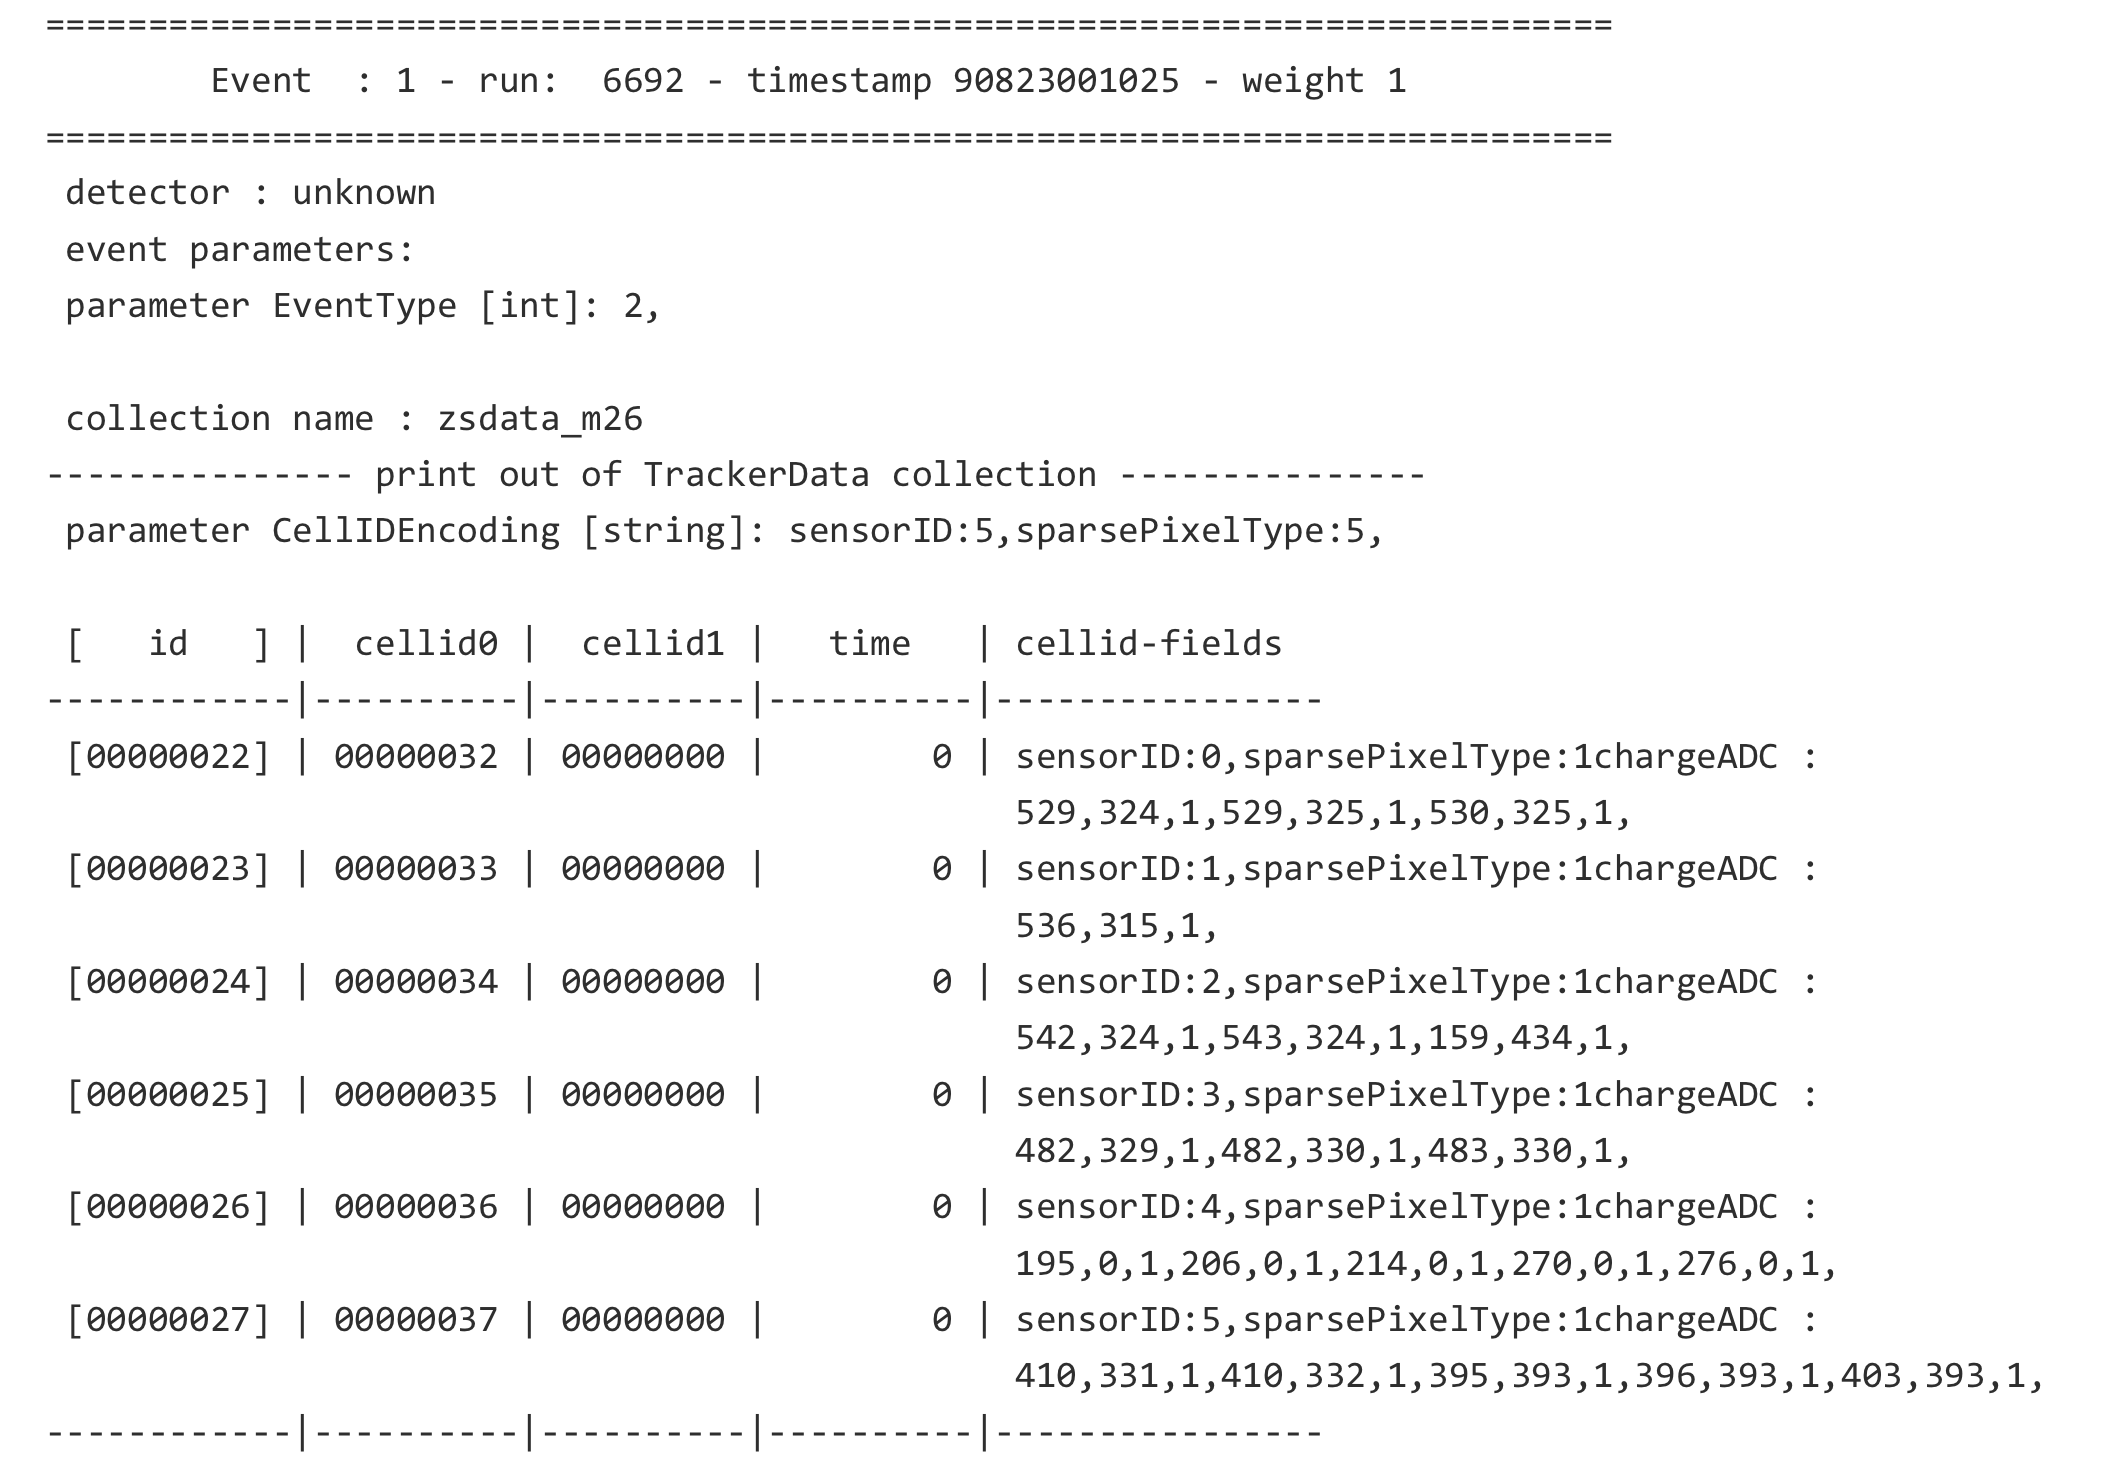
\includegraphics[scale=0.4]{dumpevent.png}
	\caption{\textit{Sample dumpevent output.}}
\end{figure}

\subsection{Anajob and lcio\_event\_counter}
\paragraph{}
Another useful tool in the toolbox of the \textit{EUTelescope} user is \textit{anajob}. \textit{anajob} is similar to \textit{dumpevent} in that it allows you to inspect your \textit{.slcio} files, however the outputs from the two tools differ slightly.
\paragraph{\textit{anajob} usage}
To invoke \textit{anajob} is a very similar process to invoking \textit{dumpevent}. At the command-line type:
\begin{minted}[breaklines]{bash}
anajob my_file.slcio
\end{minted}
to inspect the file \textit{my\_file.slcio}.
\paragraph{}
With \textit{dumpevent} you get detailed information regarding exactly what values are stored in all of your collections for a given event. Whilst this is a very useful tool, the output can quickly become bloated and messy, simply because the tool outputs a lot of information. With \textit{anajob} the user gets a very similar output, but its more of an overview. \textit{anajob} will output the event header information, as well as a count of the number of objects that are stored within each collection. The image below shows a sample output from \textit{anajob}.
\begin{figure}[!ht]
	\centering
	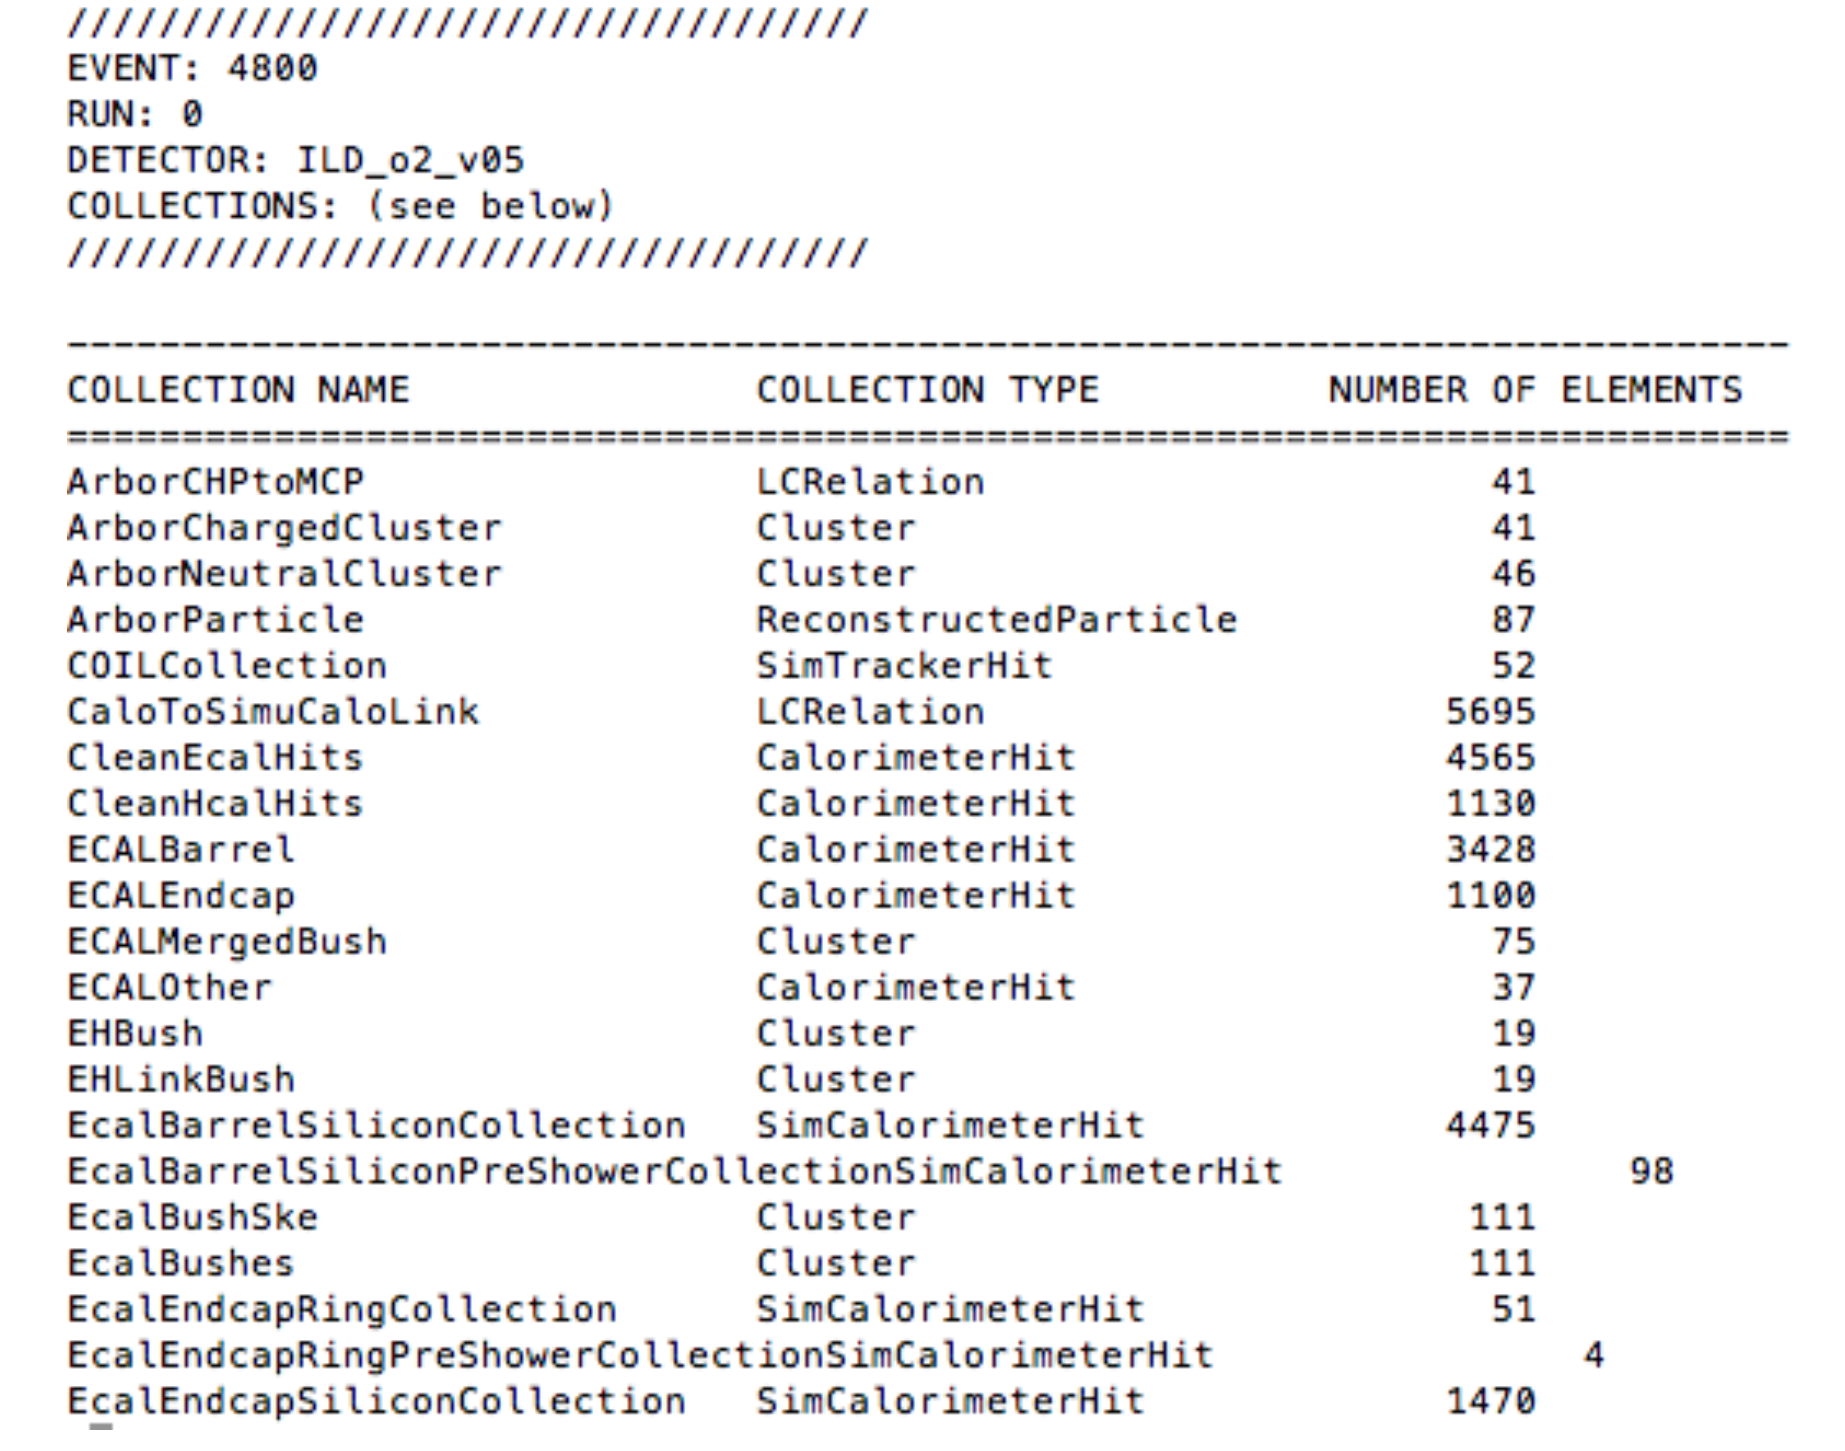
\includegraphics[scale=0.4]{anajob.png}
	\caption{\textit{Sample anajob output. Image take from [10]}}
\end{figure}
\paragraph{lcio\_event\_counter usage}
In addition to the aforementioned tools, another exists called \textit{lcio\_event\_counter}. This tool provides an even slimmer output than \textit{anajob}, showing only the number of events contained within a \textit{.slcio} file, making it useful for quick checks. Invoke it with the following command:
\begin{minted}[breaklines]{bash}
lcio_event_counter my_file.slcio
\end{minted}
\section{Worked Examples}
\paragraph{}
This section runs through basic worked examples to show new users what a simple reconstruction and analysis will look like.  This section is intended to familiarise the user with the interface that EUTelescope provides and to give the user some understanding of the key steps needed to successfully reconstruct telescope test beam data. This information can only really be considered an overview of the usage of EUTelescope because the needs of the individual user vary greatly, and as such no two analyses are the same. The examples shown below contain some of the most common steps used when analysing test beam data. They provide a good jumping off point for learning to use the software and also could form the basis of an analysis that the user wishes to pursue.
 \paragraph{}
In addition to what will be shown here, users are encouraged to go through the \textit{jobsub/examples} folder in order to familiarise themselves with the operation of the software. An excellent resource with very detailed information on \textit{jobsub} and the whole EUTelescope process can be found in the \textit{jobs/README} file located at the following directory:
\begin{minted}[breaklines]{bash}
/ilcsoft/v01-17-05/Eutelescope/trunk/jobsub
\end{minted}
\paragraph{}
The next part of this guide will look at using the \textit{Aconite4Chip-local} example.
\subsection{Aconite4Chip-local}
\paragraph{}
The Aconite4Chip-local example is a good choice for a first analysis due to its simplicity. To being the analysis, navigate to the following location and source the \textit{build\_env.sh} script as follows:
\begin{minted}[breaklines]{bash}
cd path/to/your/ilcsoft/vxx_yy/EUTelescope/trunk/
source build_env.sh
\end{minted}
This will initialise all of the environment variables required to set up and use EUTelescope. If you are using EUTelescope on one of the pre-installed virtual machines then the full path is:
\begin{minted}[breaklines]{bash}
/home/eutel/ilcsoft_eutel/v01-17-05/Eutelescope/trunk/
\end{minted}
You can check that the environment has initialised properly by typing:
\begin{minted}[breaklines]{bash}
echo $EUTELESCOPE
\end{minted}
into your terminal. If everything is working as expected then it should return the path to your EUTelescope repository, which should be the current working directory.
\paragraph{}
From here, navigate to the Aconite-4chipLocal output folder in the jobsub directory:
\begin{minted}[breaklines]{bash}
/ilcsoft_eutel/v01-17-05/Eutelescope/trunk/jobsub/examples/aconite-4chipLocal/output
\end{minted}
\paragraph{}
Once in the output folder, 4 directories need to be made. These are \textit{database, histograms, lcio, logs}. These folders will be used by EUTelescope to stash the output of various processors used throughout the analysis chain. Create these folders, and then change directory to the folder above, by typing:
\begin{minted}[breaklines]{bash}
mkdir -p database histograms lcio logs
cd ../
\end{minted}
\paragraph{}
The current working directory is the working directory for the analysis. There are 2 important files to be noted in here; \textit{config.cfg} and \textit{runlist.csv}. The config file outlines the whole analysis. Open it up with a text editor to get an understanding of what it details. If you are unaware of what config files contain then please read section 3.4.3. 
\paragraph{}
Reading through the file and recalling that the required processors names are contained within ``[]'', it is possible to see that the following steps, or processors are needed to complete the analysis:
\begin{enumerate}
\item Converter
\item Clustering
\item Hitmaker
\item Alignment
\item Fitter
\end{enumerate}
\paragraph{}
The config file also contains all of the key file paths for the software to make use of during the analysis. It tells EUTelescope: what the base path is, where to find the RAW EUDAQ data files, where to find the steering files, GEAR files etc. It also contains the values for some important analysis parameters that are used during the execution of the processor. The runlist file contains run-specific parameters that need to be given to EUTelescope, parameters such as beam energy for instance.
\paragraph{Converter}
The task of EUTelescope is to reconstruct raw EUDAQ data into particle tracks and so the first stage of this analysis, and most analyses, is to convert the EUDAQ RAW files into something readable by EUTelescope, and this is achieved by the \textit{Converter} processor. To run this step make sure that the EUDAQ RAW files are in the location defined by the \textit{NativePath} variable in the config file. Often the files are located in an AFS directory so AFS must be configured on your machine prior to use. If AFS is not an option then the RAW files can be made copied to a local directory. Users of the virtual machines might find it useful to create a second virtual hard drive and add it to the VM. All the RAW files could then be stored on the secondary virtual drive and read into EUTelescope from there.
\paragraph{}
Some test data to use with the walk through can be found at the following AFS directory:
\begin{minted}[breaklines]{bash}
/afs/desy.de/group/telescopes/EutelTestData/TestExampleAconiteQuadFEI4
\end{minted}
\paragraph{}
For the purpose of this walk through a raw file called \textit{run001085.raw} was used.
\paragraph{}
Once everything is set up correctly, execute the converter step from the Aconite-4chipLocal base directory with the following command:
\begin{minted}[breaklines]{bash}
jobsub -c config.cfg -csv runlist.csv converter 1085
\end{minted}
Where the 4 digit number at the end indicates the run number to be processed. Note that jobsub commands always follow this general format as outlined in section 3.4.1.
\paragraph{}
It is also possible to break the above command down into two steps. By adding the option \textit{--dry-run} to the command, Marlin does not get executed but a steering file to be used by the processor gets created from the tempory steering files located in the \textit{steering-templates} folder. Marlin can then be executed separately with the newly created steering file. This is achieved with the following two commands:
\begin{minted}[breaklines]{bash}
jobsub -c config.cfg -csv runlist.csv --dry-run converter 1085
Marlin converter-001085.xml
\end{minted}
Where \textit{converter-001085.xml} is the newly created steering file that has been created from the template steering file. Breaking the command down into two steps as shown above provides some insight into what \textit{jobsub} is actually doing. It is collating all the relevant information the config file and the runlist and then it is writing this information into a steering file. It then automatically takes that steering file and executes Marlin with it.
\paragraph{}
Upon completion of this step we are left with a \textit{run001085-converter.slcio} file which contains all the information from the \textit{run001085.raw} converted into the .slcio event based file format. This file will get written to the \textit{output/lcio} directory, as will all of the produced .slcio files.
\paragraph{Clustering}
After the file conversion stage is complete the next step in the Aconite-4chipLocal reconstruction is the clustering step. This step analyses hit clusters in the data and removes clusters that are fake due to causes such as a pixel firing too often; this makes it appear as if the telescope has registered a hit from the beam when in fact it has not. Running the clustering stage is simple and follows the same idea as running the converter stage. Type in the following command to execute the clustering process:
\begin{minted}[breaklines]{bash}
jobsub -c config.cfg -csv runlist.csv clustering 1085
\end{minted}
\paragraph{}
Again, as with the converter step, it is possible to separate these commands into two steps like so:
\begin{minted}[breaklines]{bash}
jobsub -c config.cfg -csv runlist.csv --dry-run clustering 1085
Marlin clustering-001085.xml
\end{minted}
\paragraph{}
Again, this will populate the steering file (called \textit{converter-001085.xml} to be used by Marlin for execution. Open up \textit{converter-001085.xml} in a text editor to see what it contains. The processors listed within the \textit{$<$execute$>$...$<$/execute$>$} tags tell Marlin what processors to invoke in what order to complete the clustering step.
\paragraph{}
Once the clustering step has successfully completed three output files will have been produced. The first one is a newly updated \textit{.slcio} file, which will contain the new data collections produced by the clustering stage. The second new file is a \textit{.root} file containing histograms. This \textit{ROOT} file can be opened by invoking ROOT and then creating a \textit{TBrowser} object from the \textit{ROOT} command line:
\begin{minted}[breaklines]{bash}
root -l run001085-clustering-histo.root
TBrowser b
\end{minted}
\paragraph{}
Once looking inside the \textit{ROOT} file it is possible to see histograms containing information about the clusters found on both the telescope planes and the DUT itself. The histograms include plots such as the total cluster size, as well as hit maps, and shown in the graphic below. These plots will provide vital information about the quality of the data and will assist with the analysis moving forward.
\begin{figure}[!ht]
	\centering
	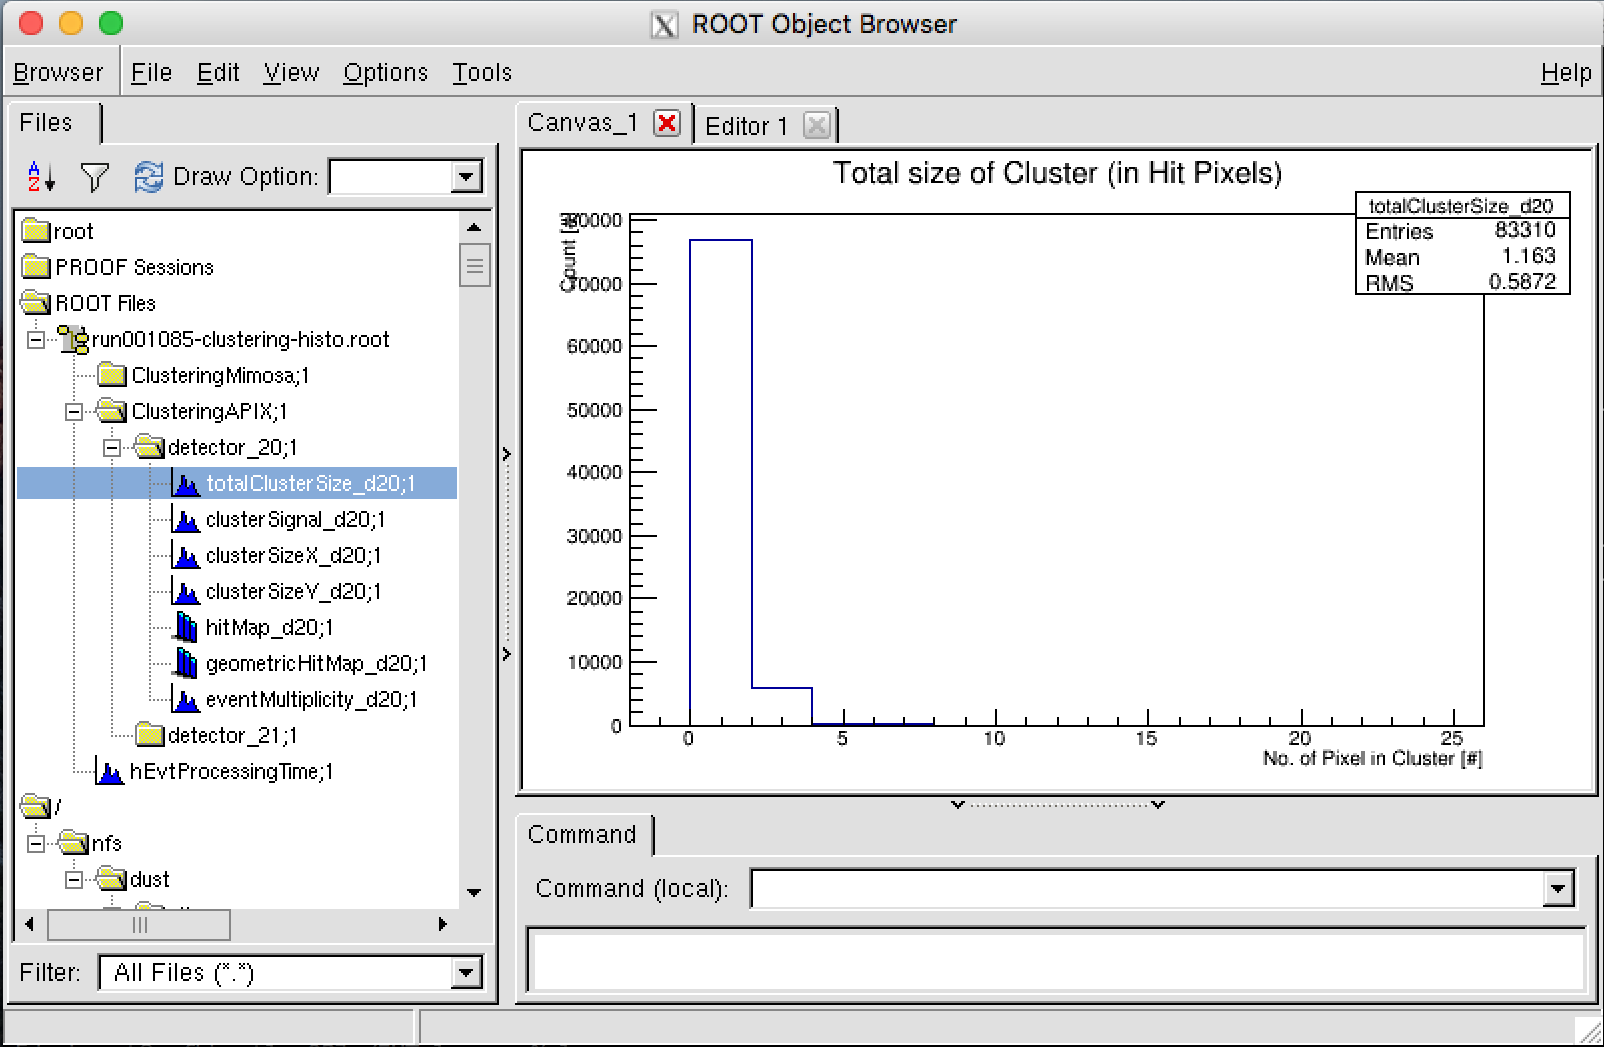
\includegraphics[scale=0.4]{clustering_totalclustersize.png}
	\caption{\textit{A plot showing the total cluster size of the data from run 1085, as viewed through a TBrowser object.}}
\end{figure}
\begin{figure}[!ht]
	\centering
	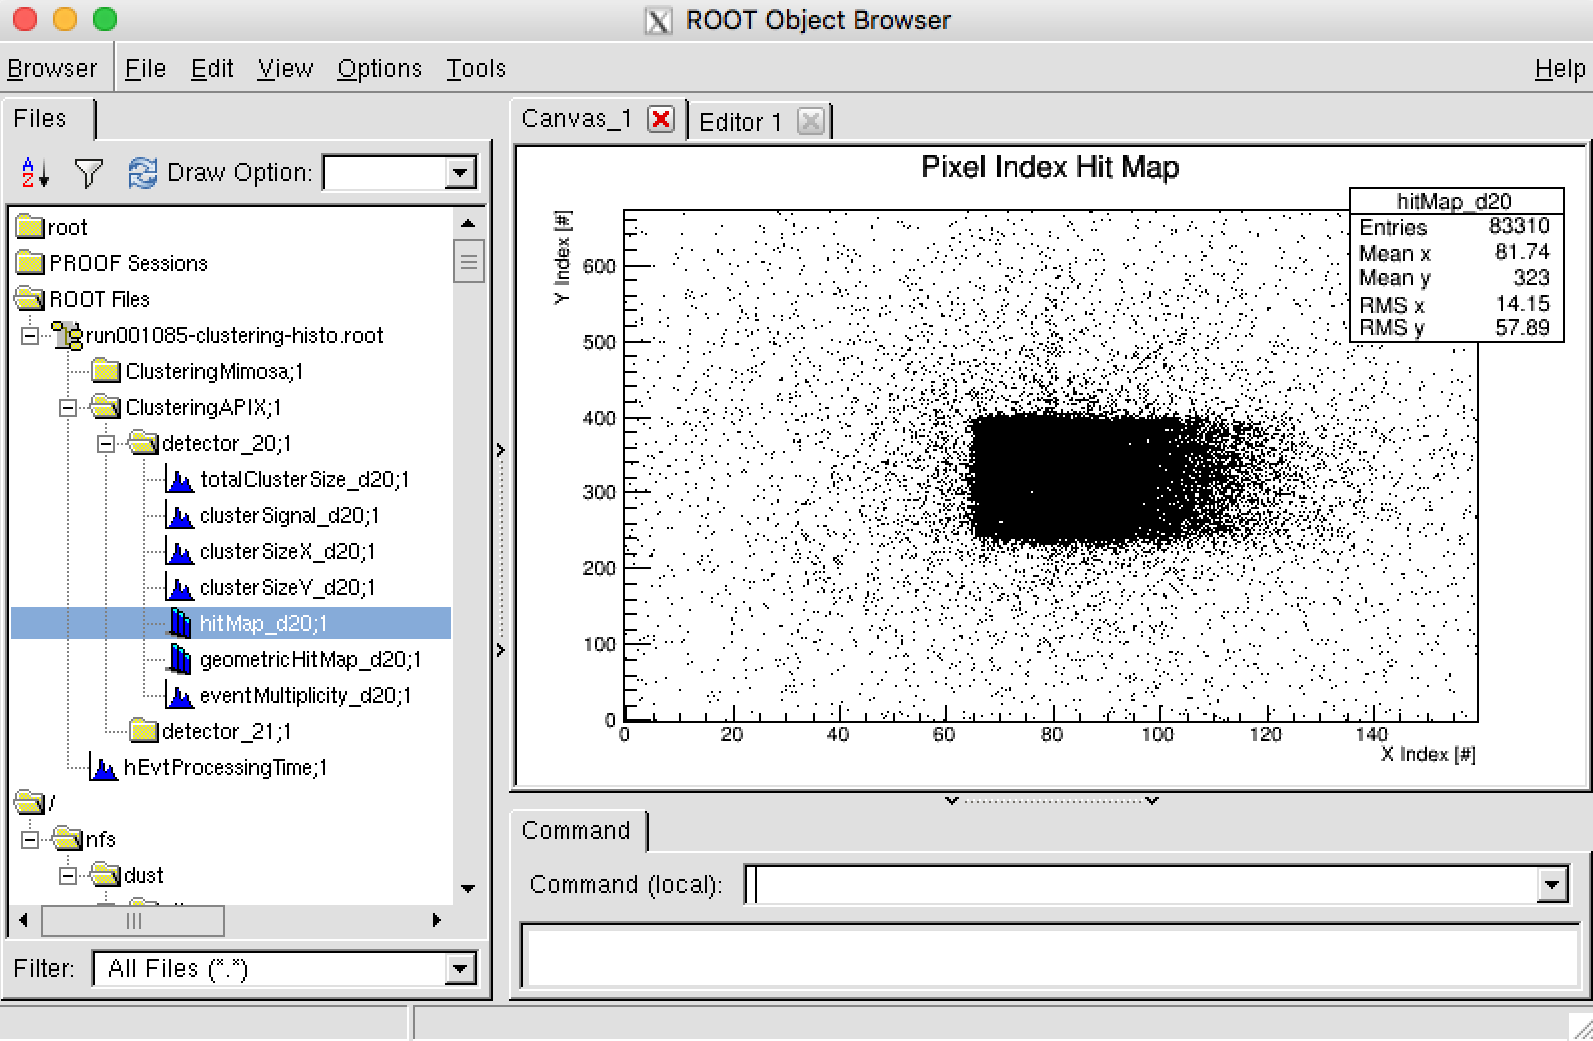
\includegraphics[scale=0.4]{clustering_hitmap.png}
	\caption{\textit{A plot showing a hitmap of the DUT plane from run 1085, as viewed through a TBrowser object.}}
\end{figure}
\paragraph{}
Additionally, a hotpixel database file will have been produced in the \textit{output/database} folder. This file contains information on which pixels have fired too often to be considered real data, and so are considered noise. The exact criteria as to what defines a pixel that fires too often can be described in the config file.
\paragraph{Hitmaker}
The \textit{hitmaker} step will analyse the information from the clustering step output and, based on selection criteria that can be altered in the config file, forms valid hit objects. Hit objects indicate the reconstructed position of a particle hit on the DUT or telescope. The crucial part of the \textit{hitmaker} step is that it takes the clusters, which are recorded in the planes local reference frame and converts the positions to the reference frame of the whole telescope. This means that all hits made by the \textit{hitmaker} step are defined on a global coordinate system and hence they are easily comparable; this is important for the next step, which is \textit{alignment}. In order to make this coordinate system transformation, Marlin will also require information contained within the setups \textit{GEAR} file. This file will contain the geometry description of the set up which describes where the sensor planes are, where the DUT is, the sizes of all the planes are and which parts of the setup are sensitive detector volumes and which parts are mechanical support structure.
\paragraph{}
To perform the \textit{hitmaker} step, invoke \textit{jobsub} in the following way:
\begin{minted}[breaklines]{bash}
jobsub -c config.cfg -csv runlist.csv hitmaker 1085
\end{minted}
\paragraph{}
Again, this step can be broken down further into two steps, if you wish to inspect the steering file to be executed by Marlin, to gain some insight into the system.
\paragraph{}
Now navigate to the \textit{output/histograms} directory and open up \textit{run001085-hitmaker-histo.root} with \textit{ROOT}. This file contains the new histograms that were produced during the \textit{hitmaker} step. The main histograms to note while looking through this file are the hitmaps for each plane and the DUT. There will be two histograms for each plane: one showing the hits in the detector reference plane and the other showing the hits in the telescope reference plane. The figure below shows both of these hit maps for the most upstream (closest to the beam outlet) plane of the telescope.
\newpage
\begin{figure}[h!]
	\begin{minipage}{0.5\textwidth}
		\centering
		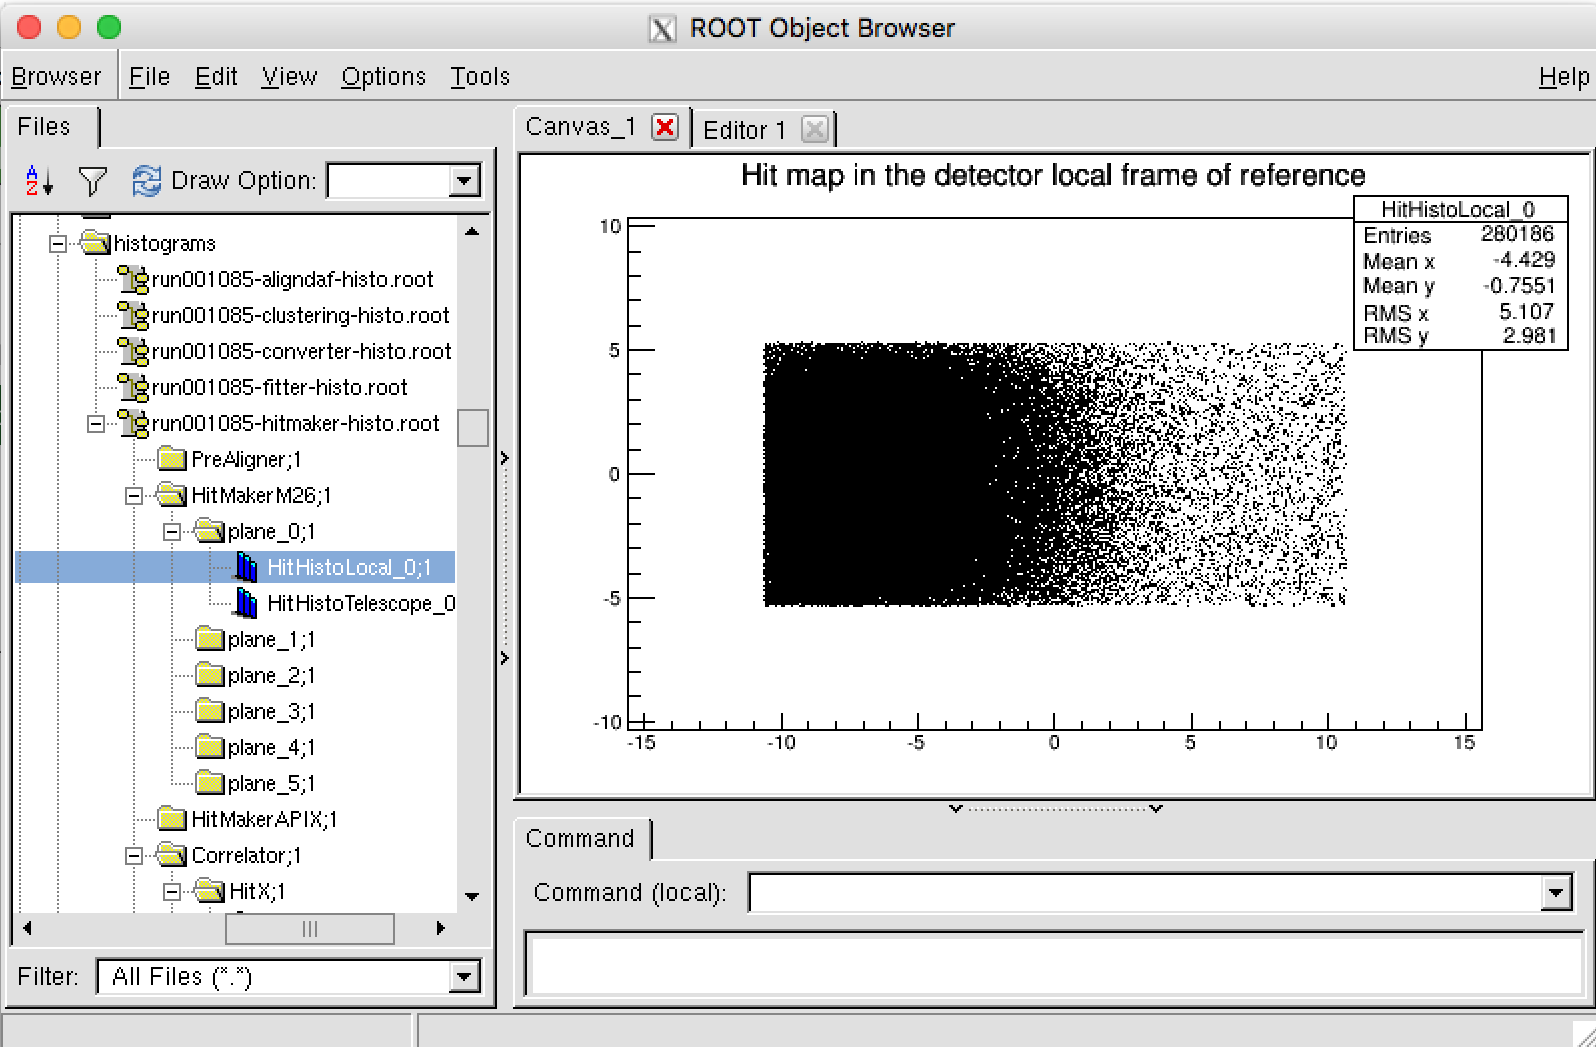
\includegraphics[scale=0.3]{hitmaker_local.png}
	\end{minipage}
    \begin{minipage}{0.5\textwidth}
		\centering
		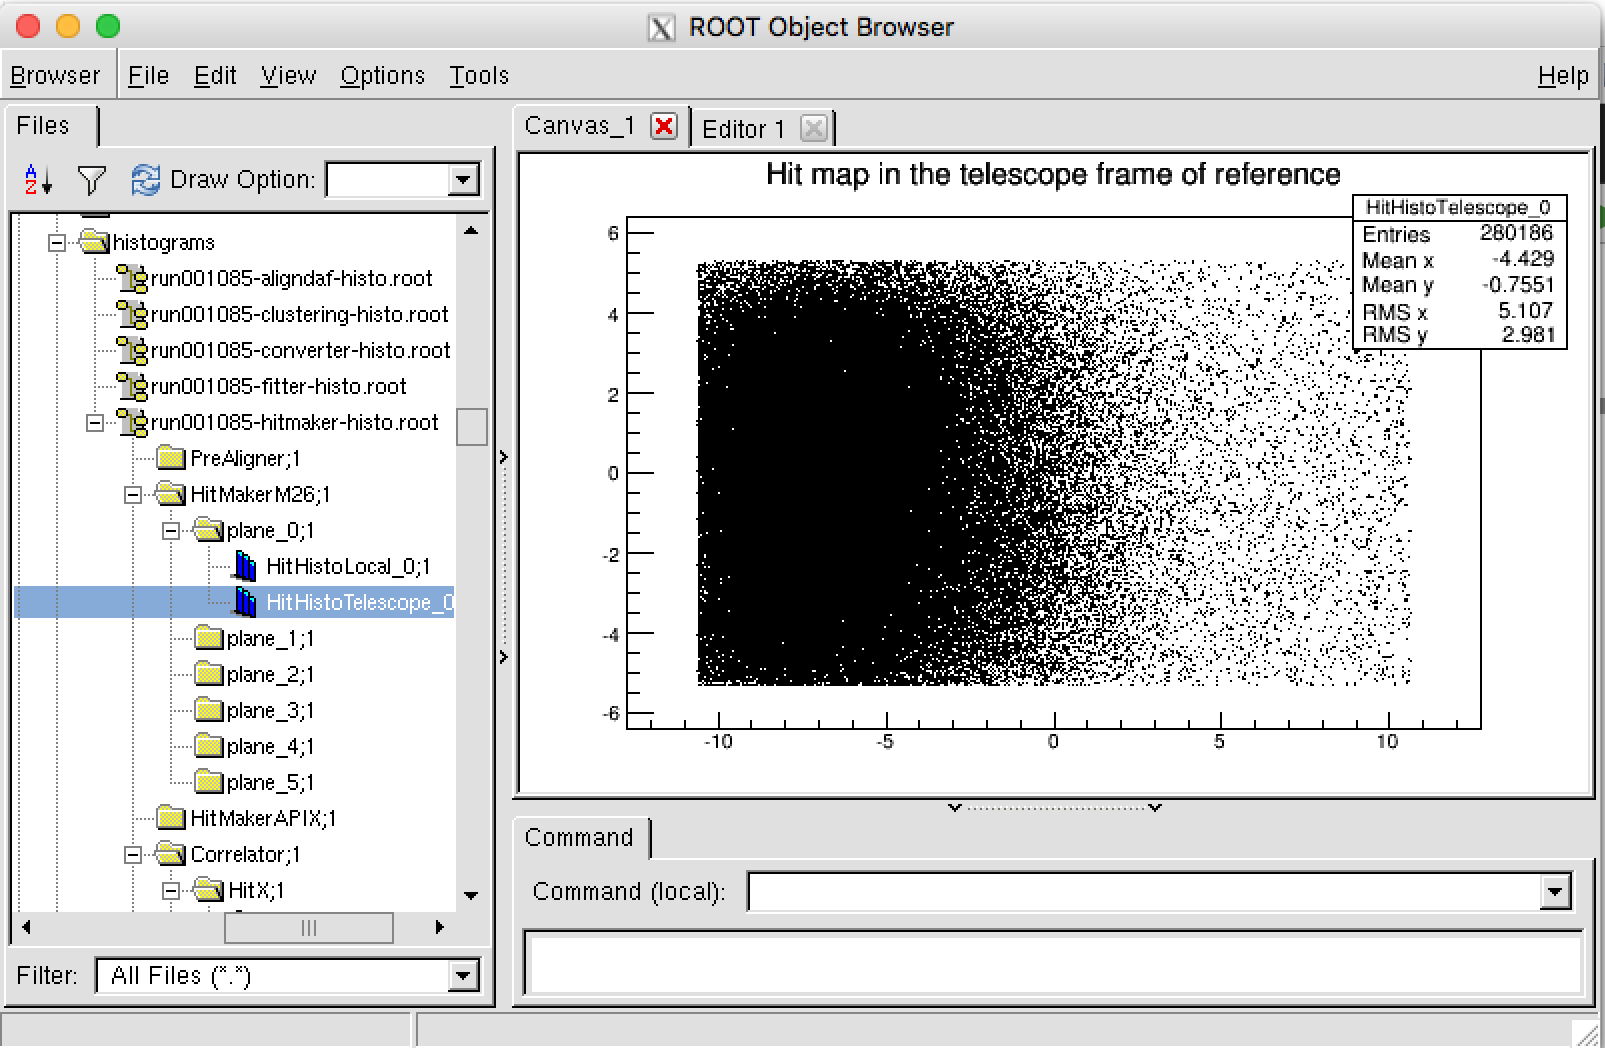
\includegraphics[scale=0.3]{hitmaker_telescope.png}
	\end{minipage}
	\caption{\textit{The image on the left shows the hits in the local detector frame and image on the right shows the same hits transformed into the global telescope reference frame. The histograms are shown as viewed through a TBrowser.}}
    \label{HVSV1}
\end{figure}
\paragraph{}
Another important set of plots to note are the correlation plots. These plots show how the $x$ (or other) coordinates between two planes line up (or correlate) with each other. The figure below shows such a plot. Note that if the set up is well aligned then one expects to see a $y=x$ distribution of the points (where $y$ and $x$ are the names given to the vertical and horizontal axes respectively, not the name of the telescope coordinates). The more points that deviate away from this trend line, the worse aligned the setup is.
\begin{figure}[!ht]
	\centering
	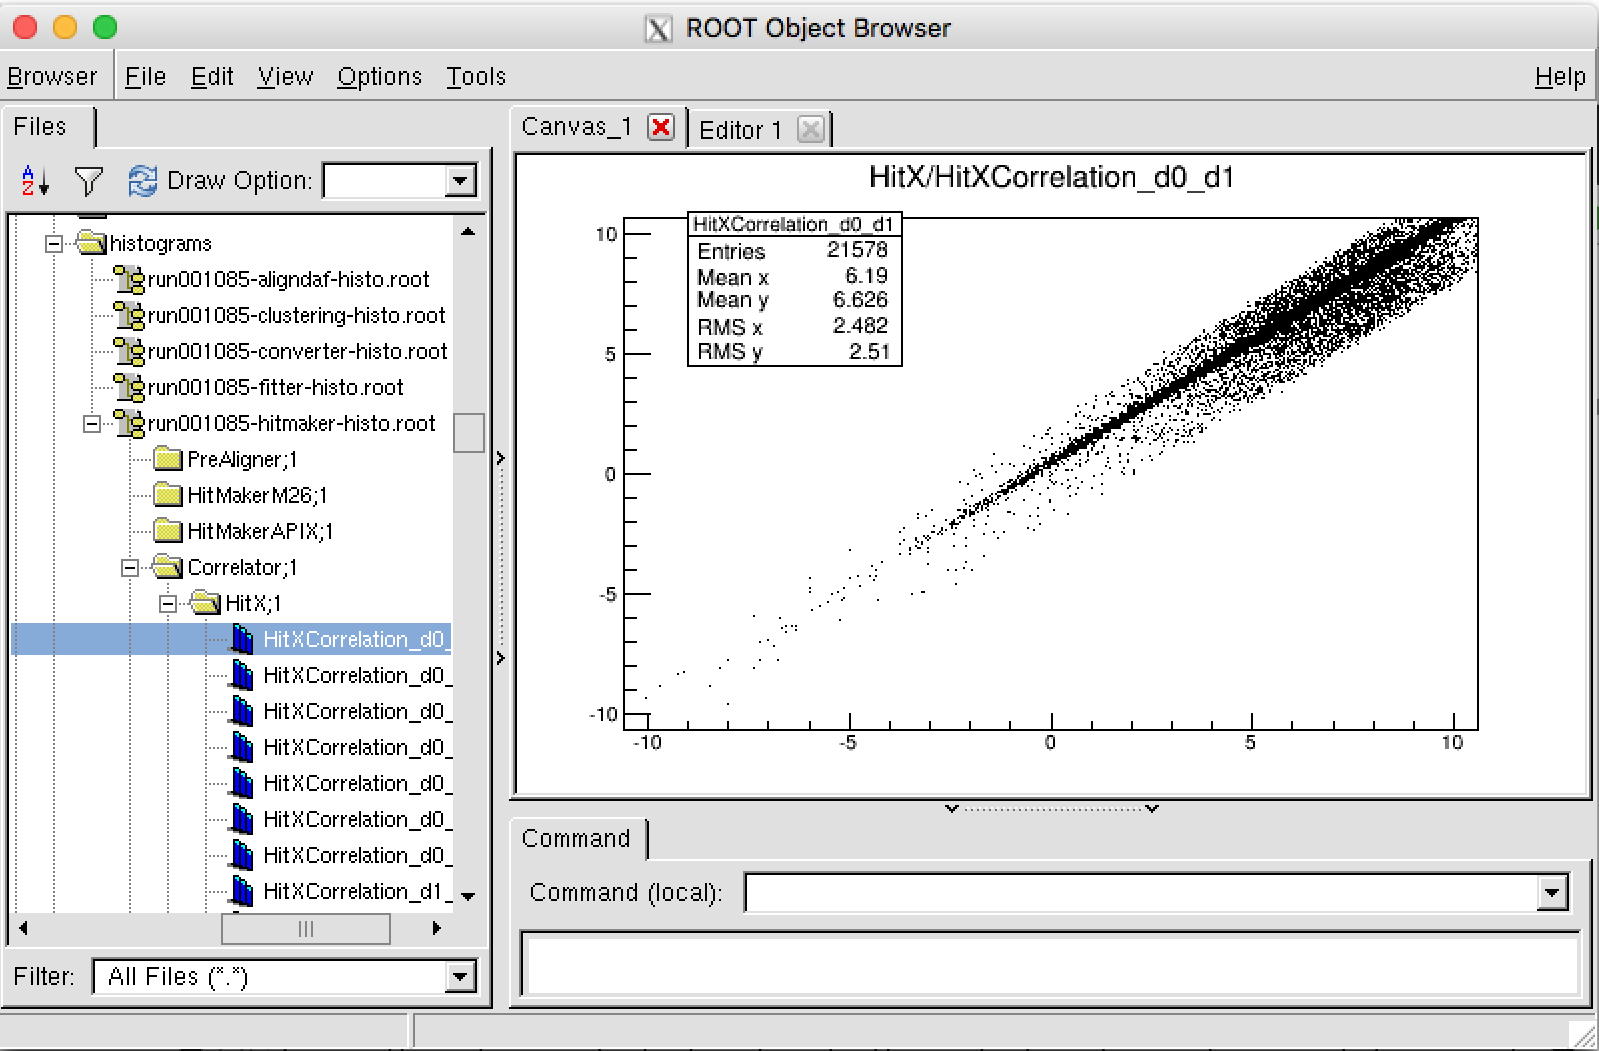
\includegraphics[scale=0.4]{hitmaker_corr.png}
	\caption{\textit{A correlation plot showing the correlation between the $x$ coordinate on the 0th and 1st planes of the telescope.}}
\end{figure}
The conclusion to draw from this particular plot is that these coordinates are fairly well aligned.
\paragraph{Alignment}
The \textit{alignment} step is a hugely important part of the reconstruction and analysis. It looks at the global hit positions, and tries to draw a straight line through a set of six hits (assuming the track in question is incident on all six telescope planes). It then looks at the residuals between the hit positions and the fit line and makes small shifts to the global position of each telescope plane. After making these shifts, it will then re-examine the residuals to see if they have decreased. This iterative process repeats and performs many shifts until an optimal fit is found. These new telescope plane positions are then written to a new database file, and that is used in conjunction with the GEAR file so that the correct positions telescope and DUT positions are used going forward.
\paragraph{}
To execute the \textit{alignment} step, use the following command:
\begin{minted}[breaklines]{bash}
jobsub -c config.cfg -csv runlist.csv align 1085
\end{minted}
The result of the alignment step is a new database files and can be found in the \textit{output/database} locations. A new set of histograms are also produced, and in this case are written to a root file called \textit{run001085-aligndaf-histo.root}. In this case the user is encouraged to open up the \textit{ROOT} file and investigate the contents. The file contains many different histograms providing information on the fits that have been performed as well as information on the residuals between various quantities.
\paragraph{Fitter}
The final step of the \textit{Aconite-4chipLocal} reconstruction is the \textit{fitter} step. This step will produce the histograms detailing the tracks, written to a \textit{ROOT} file in the usual way.
\paragraph{}
To execute the \textit{fitter} step, type the following into the terminal:
\begin{minted}[breaklines]{bash}
jobsub -c config.cfg -csv runlist.csv fitter 1085
\end{minted}
\paragraph{}
The successful completion of this step produces the aforementioned \textit{ROOT} file called \textit{run001085-fitter-histo.root}. Again, the user is encouraged to investigate the histograms produced at this stage. If this were a real analysis then the histograms that are produced by this stage are the final products that are produced by reconstructing telescope data with EUTelescope. These histograms will then be the subject of further study to ascertain the performance of the DUT, or whatever the original aim the test beam was.
\paragraph{}
Also produced by the \textit{fitter} stage is an LCIO collection of track objects stored in a \textit{.slcio} file. This file can then be processed by user written code created using the LCIO software framework. Detailed analysis of the test beam data can be performed using this file.
\paragraph{}
This completes the walk through of the Aconite-4chipLocal reconstruction procedure.
\subsection{datura-noDUT}
\paragraph{}
A second analysis walk through is also provided in this section. This section is described in less detail and is intended to be run after a successful completion of the \textit{Aconite-4chipLocal} example for new users. Treat this as an opportunity for solidifying your knowledge of EUTelescope after having learned the basics with the first example walk through.
\paragraph{}
A raw data file for use in the \textit{datura-noDUT} example can be found in at the following AFS directory:
\begin{minted}[breaklines]{bash}
/afs/desy.de/group/telescopes/EutelTestData/TestExampleDaturaNoDUT/
\end{minted}
\paragraph{}
Once the data file has been collected, make sure that the \textit{NativePath} variable in the config file points to the correct directory. If you are connecting to the file with AFS then you will not need to alter this value.
\paragraph{}
For this reconstruction the following steps are needed:
\begin{enumerate}
\item Converter
\item Clustering
\item Filter
\item Hitmaker
\item Alignment
\item Fitter
\end{enumerate}
\paragraph{}
To begin the analysis change directories to the \textit{datura-noDUT} base directory (this is defined in the config file). The following jobsub commands are everything needed to run the analysis on the example run file, number 97.
\begin{minted}[breaklines]{bash}
jobsub -c config.cfg -csv runlist.csv converter 97
jobsub -c config.cfg -csv runlist.csv clustering 97
jobsub -c config.cfg -csv runlist.csv filter 97
jobsub -c config.cfg -csv runlist.csv hitmaker 97
jobsub -c config.cfg -csv runlist.csv align 97
jobsub -c config.cfg -csv runlist.csv fitter 97
\end{minted}
\paragraph{}
Run through the reconstruction process paying attention to the outputs produced at each stage. Remember that it is possible to add the option \textit{--dry-run} to all of the above commands if you wish to inspect the actual steering files before they are processed by Marlin.
\section{EUTelescope Virtual Machines}
\paragraph{}
This section describes and details the VirtualBox Virtual Machines (VMs) that have been created for use with EUTelescope. These machines have been put together in order to enable users who have difficulty with the installation process to be able to get up and running quickly with their data analysis and reconstruction.
\paragraph{}
Currently, there are 2 distinct machines available. The first is a standard installation of EUTelescope, which will install the ``trunk'' version from the Github repository. The other machine is a very specific setup for use by the ITk strips subcollaboration within ATLAS. This machine uses the latest version of EUTelescope, but with EUDAQ version 1.7-dev (as well as v1.4.5 and v1.6.0).
\subsection{Installing VirtualBox}
\paragraph{}
In order to run the VM, the user must first download and install VirtualBox. This is very straight forward and more information can be found at this link: \url{https://www.virtualbox.org}.
\subsection{Retrieval of the VirtualBox VM folder}
\paragraph{}
Now that VirtualBox is installed, the next step is to download the VM folder that contains the VM you wish to run. As mentioned previously there are two distinct virtual machine builds available: standard and strips. You must make sure you are downloading the version that you require.
\paragraph{}
Although VirtualBox is fully cross-compatible, the methods used to zip the VM folders are not. As such, there are three differently zipped versions of each of the two available VMs. There are currently .tgz (Linux), .zip (OSX) and .7z (Windows) archives available. The links for the different versions are provided below. Please send an email to \textit{thomas.daubney@desy.de} if you have any problems with downloading.
\begin{enumerate}
\item Standard installation
\begin{description}
\item [Linux] \url{https://desycloud.desy.de/index.php/s/1AWQ5eSg39RFEXF}
\item [OS X] \url{https://desycloud.desy.de/index.php/s/tDQmNauHaKWXIZT}
\item [Windows] \url{https://desycloud.desy.de/index.php/s/oWq3utZq5FVGKLf}
\end{description}
\item ITk Strips installation
\begin{description}
\item [Linux] \url{https://desycloud.desy.de/index.php/s/PEtjvECFrlbX1jT}
\item [OS X] \url{https://desycloud.desy.de/index.php/s/wr0zE4sIaKVxzra}
\item [Windows] \url{https://desycloud.desy.de/index.php/s/c6mG5MC7qzKtsRG}
\end{description}
\end{enumerate}
\subsection{Adding the VM to VirtualBox and booting up}
\paragraph{}
Once you have retrieved the EUTelescope VM folder, the next step is to add it into VirtualBox, so that you can run it. VirtualBox creates a folder in the users local directory called \textit{VirtualBox VMs}, but it only creates this folder upon successful creation of the first VM using your instance of the software. If you are not already a VirtualBox user, this folder may not exist for you yet. If you have this folder then it is recommended, for neatness, to copy the EUTelescope VM folder into this \textit{VirtualBox VMs} directory. If you do not have this folder, it is not a problem; VirtualBox can add a VM from any location. Select \textit{Machine - Add} from the VirtualBox menu.
\begin{figure}[!ht]
	\centering
	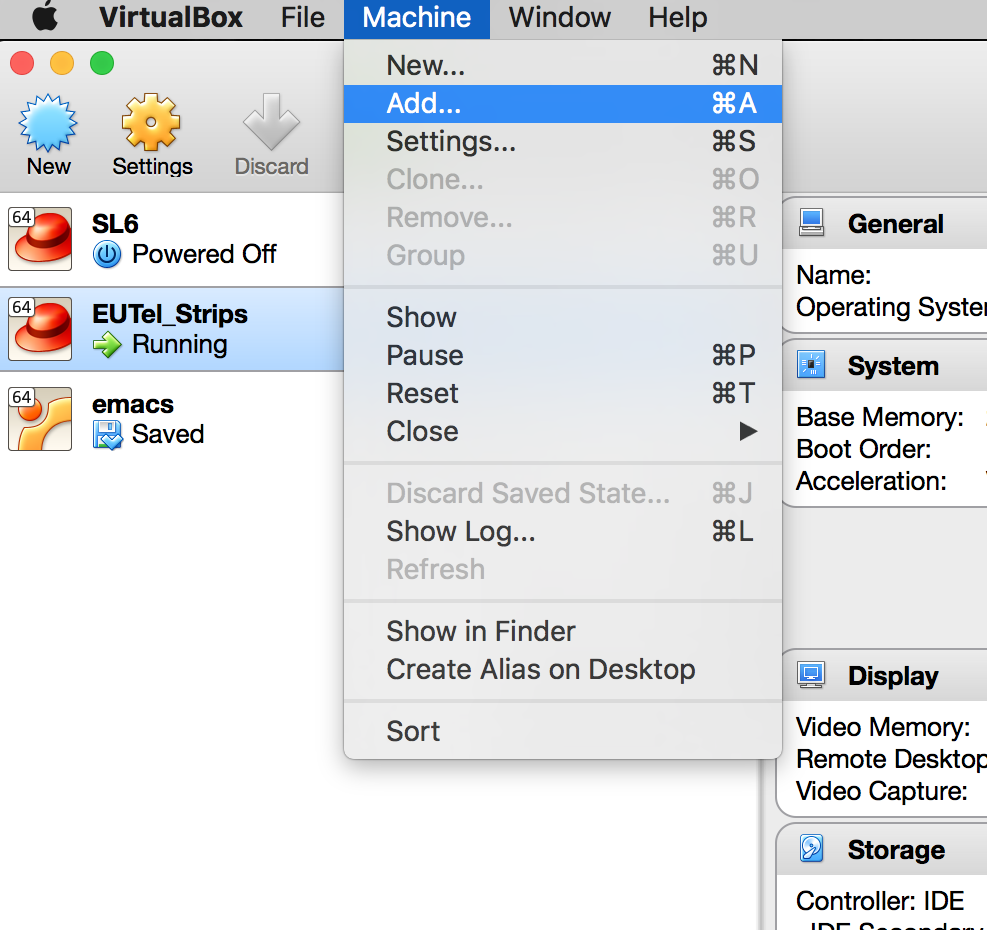
\includegraphics[scale=0.3]{addmachine.png}
	\caption{\textit{The Add Machine menu.}}
\end{figure}
\paragraph{}
navigate to the folder containing the VM. Open up this folder and locate the file shown in the image below:
\begin{figure}[!ht]
	\centering
	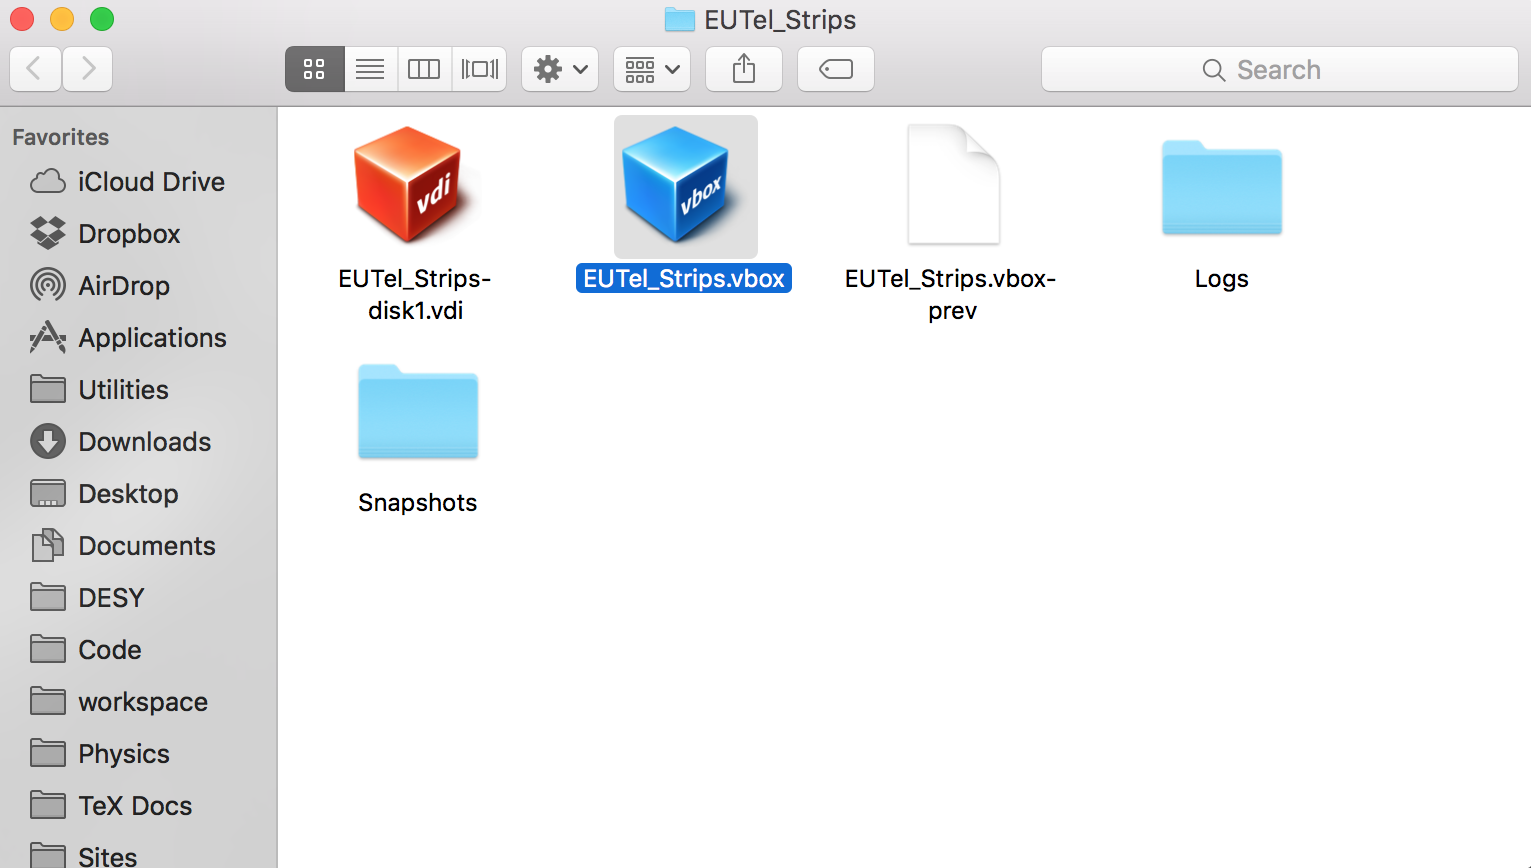
\includegraphics[scale=0.3]{vbfile.png}
	\caption{\textit{The VirtualBox file needed to add the machine.}}
\end{figure}
Double clicking the \textit{.vbox} file will then add it to your system. At this point you are ready to boot up! You can do this by selecting the machine from the list in the VirtualBox main window, and clicking \textit{Start}.
\subsection{Creating a new machine from an existing .vdi file}
Vdi files are the files used as virtual hard drives by VirtualBox VMs. If you have downloaded one of the virtual box folders from the DESY Cloud then you will have noticed that one of the files contained in those folders is a .vdi file.
\paragraph{}
Occasionally, VirtualBox will have problems simply adding in a whole virtual machine folder; it may claim that it doesn't know the location of certain files. If this happens to you, then it is straight forward to create a brand new VM within VirtualBox, and then add an existing hard drive. The following section describes how to do this.
\paragraph{Creating a new machine}
This sections assumes you have already downloaded one of the VMs from DESY Cloud, so that you have one of the correct .vdi files. If you have not done this, please see section 5.2 for information on how to retrieve the folders.
\paragraph{}
With this folder now downloaded open up VirtualBox and click on the ``New'' button, and enter the VM name and select the operating system as shown below. Note the OS for the EUTelescope VMs is Red Hat 64 (SL6).
\begin{figure}[!ht]
	\centering
	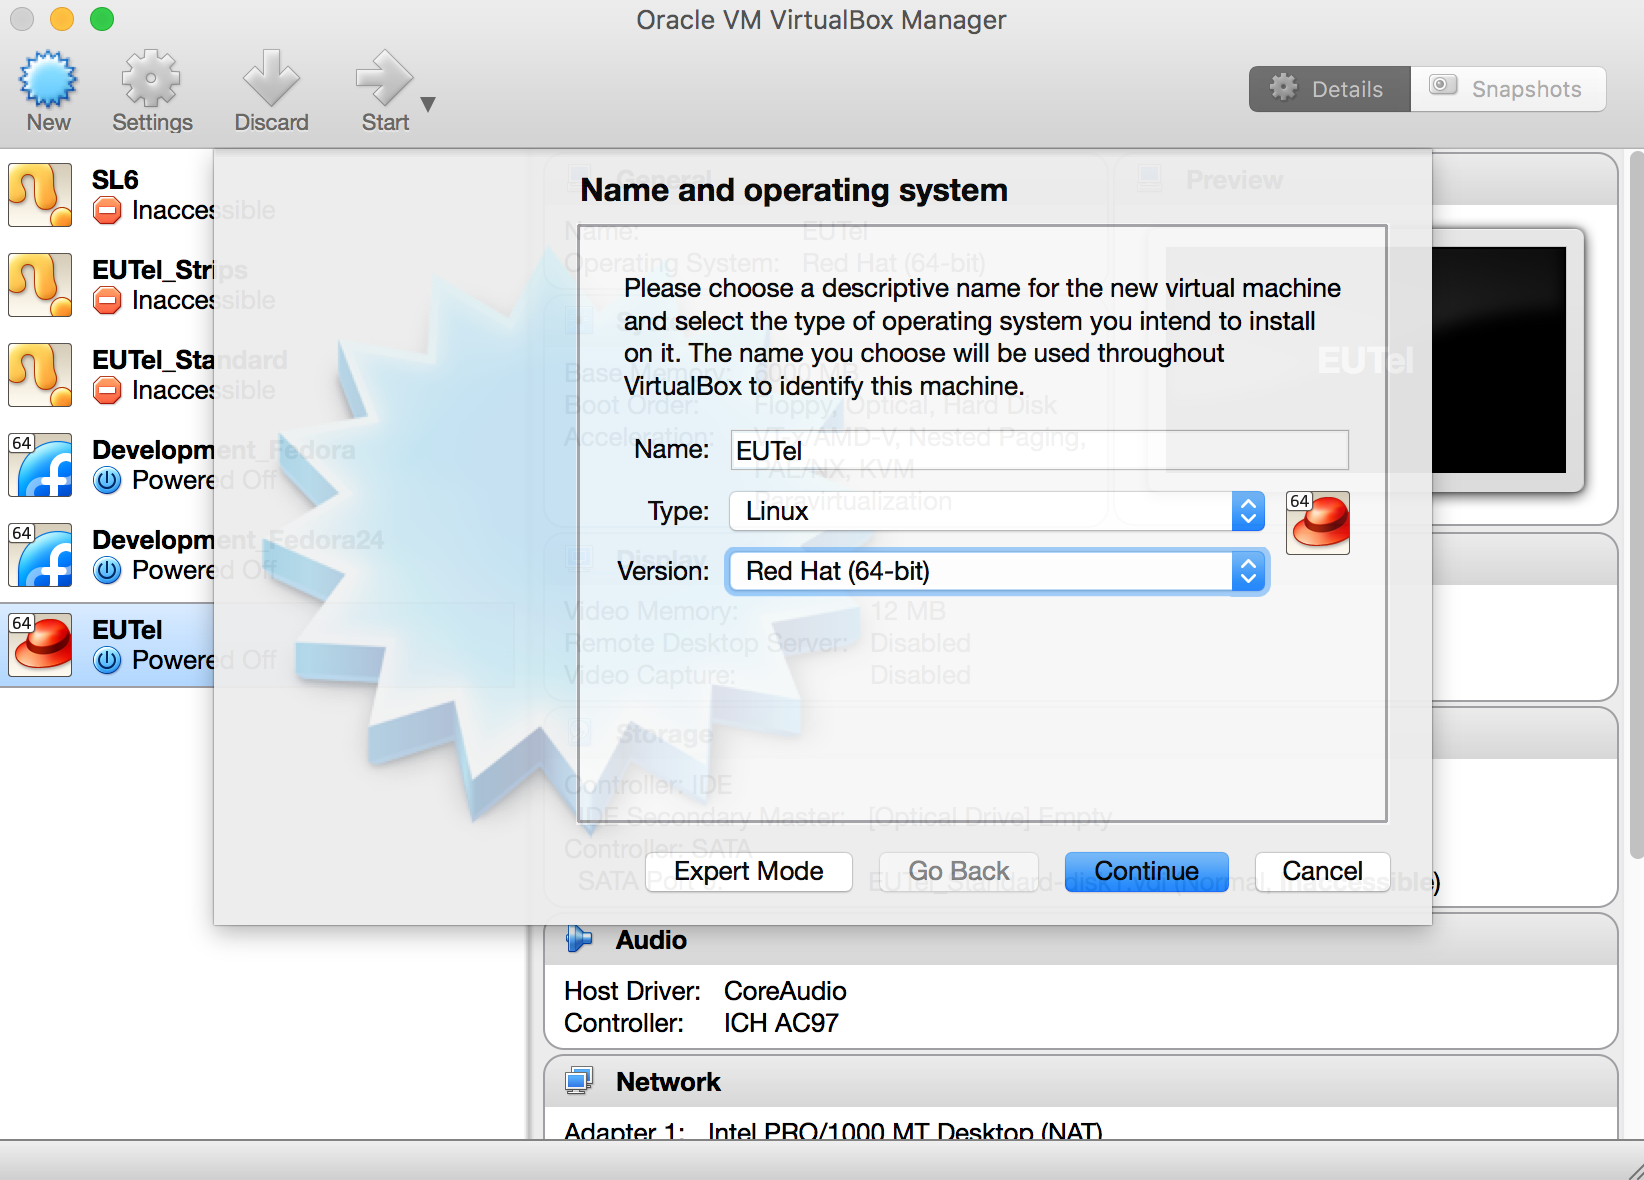
\includegraphics[scale=0.3]{new_pc.png}
	\caption{\textit{The New VM menu.}}
\end{figure}
\paragraph{}
Once this data is input, click ``Continue'' and select the desired amount of RAM for the new machine. Remember not to select too much RAM; you could end up not leaving your host machine with enough to run its own OS, so choose wisely.
\begin{figure}[!ht]
	\centering
	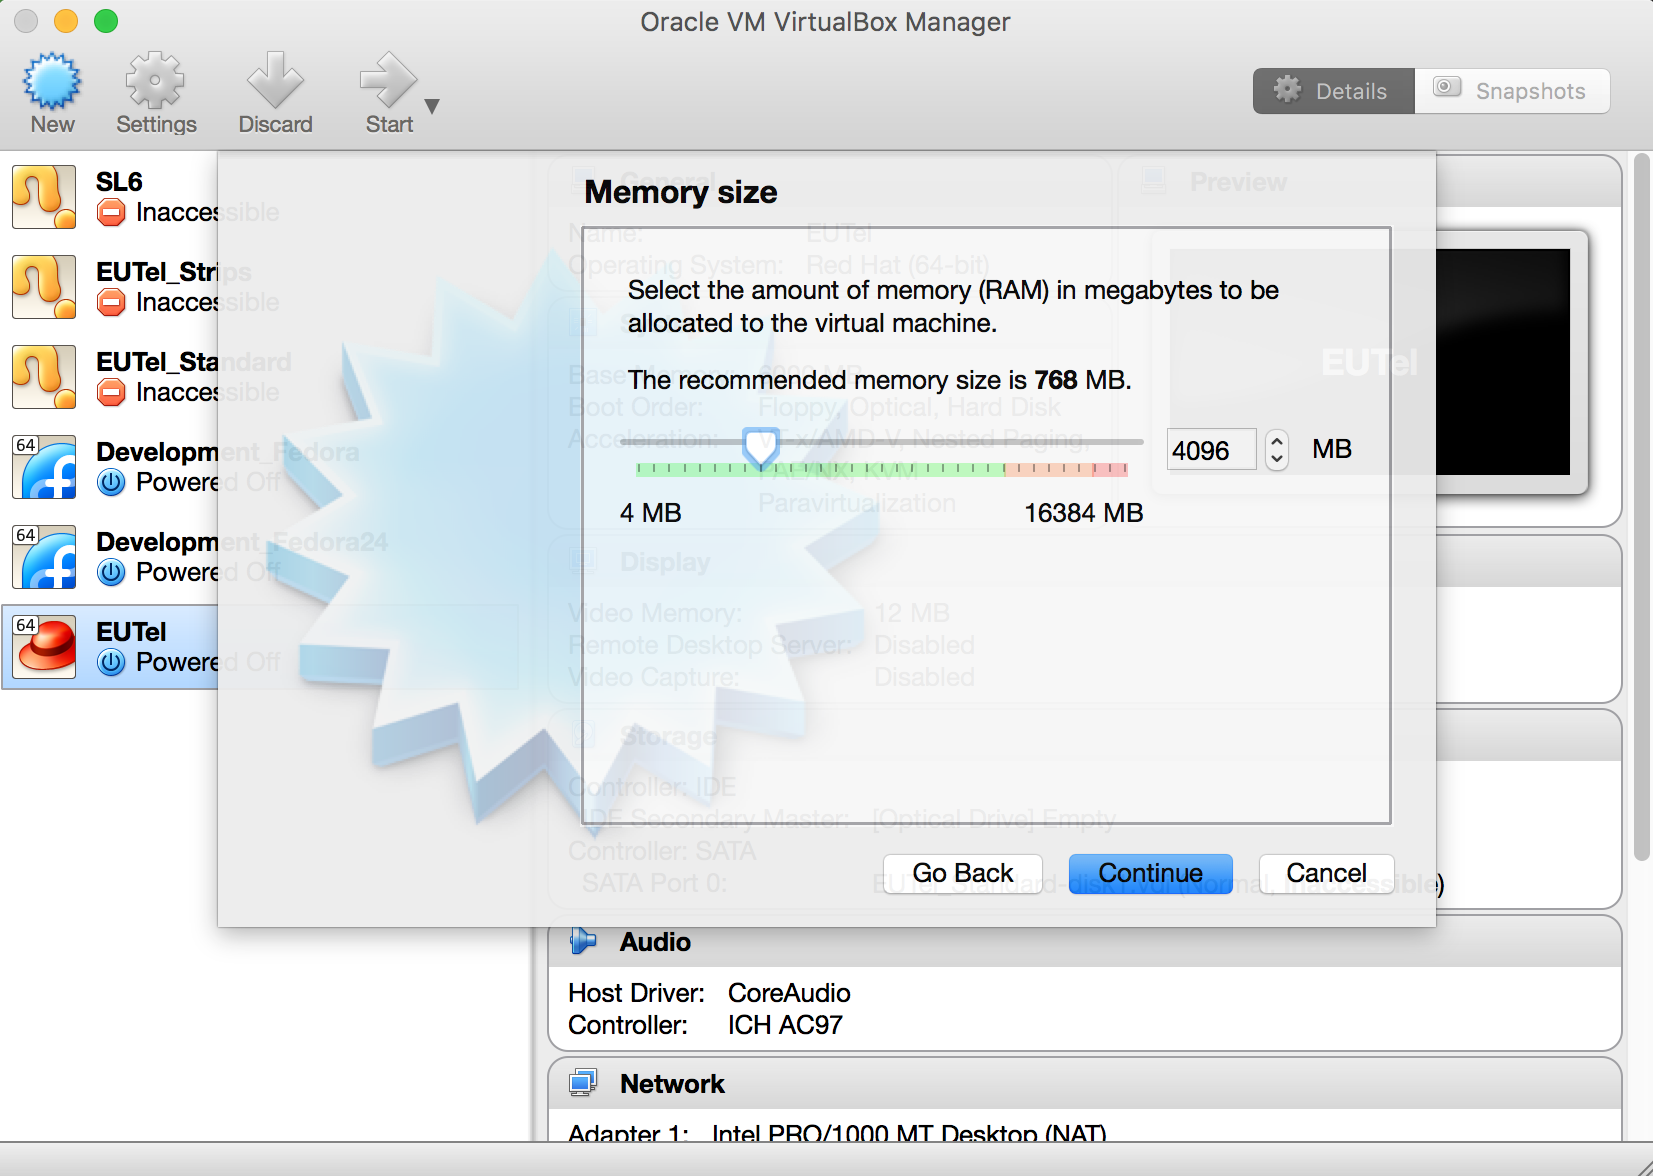
\includegraphics[scale=0.3]{choose_ram.png}
	\caption{\textit{The RAM menu.}}
\end{figure}
Once you have selected an appropriate amount of RAM click ``Continue''. At this window you want to select an existing .vdi hard drive file for virtual box to use. Using the drop down button select the .vdi you wish to use with this VM and then click ``Create''.
\begin{figure}[!ht]
	\centering
	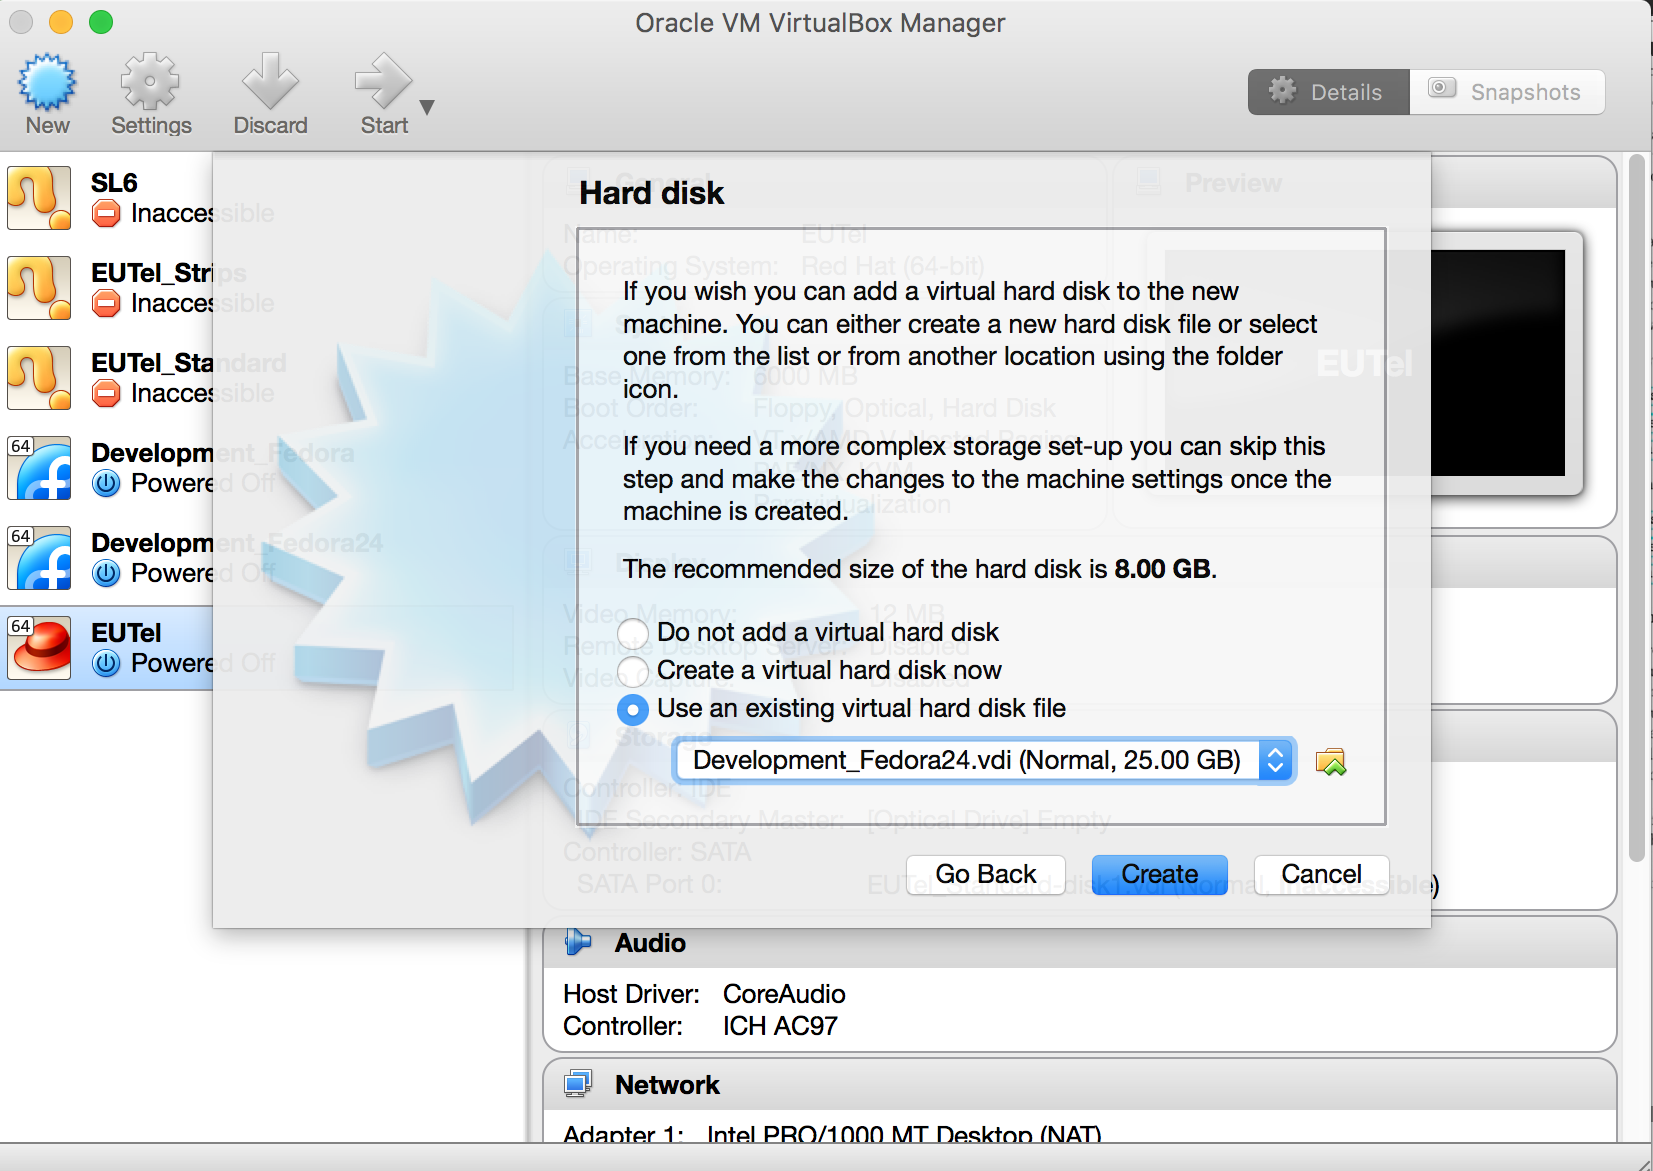
\includegraphics[scale=0.3]{add_hdd.png}
	\caption{\textit{The hard drive menu.}}
\end{figure}
\paragraph{}
This will create a new VM with an existing hard drive. Now start the VM in the normal way to use it.
\subsection{User and root credentials}
\paragraph{}
To work with the machines, the following credentials are provided:\\
\textbf{User Name:} EUTelescope\\
\textbf{Password:} eutelescope\\
\textbf{Root password:} eutelescoperoot\\
\paragraph{}
The settings in the virtual machines have been adjusted such that the user \textit{EUTelescope} does not have to enter the root password every time ``sudo'' is used. This was done by logging in as the root user and executing the \textit{visudo} command in the terminal. Executing \textit{visudo} enables the user to edit an extremely important system file, called the \textit{sudoers} file, located at \textit{/etc/sudoers}. Note that this file should never be edited directly, only via the \textit{visudo} command. The \textit{sudoers} file essentially tells the OS which users can use \textit{sudo} to execute certain commands.
\paragraph{}
Should the user dislike this behaviour of not requiring the password it can easily be changed. To do this, log in as the root user using the credentials listed above, and then type \textit{visudo} into the terminal. The image below shows what will be displayed:
\begin{figure}[!ht]
	\centering
	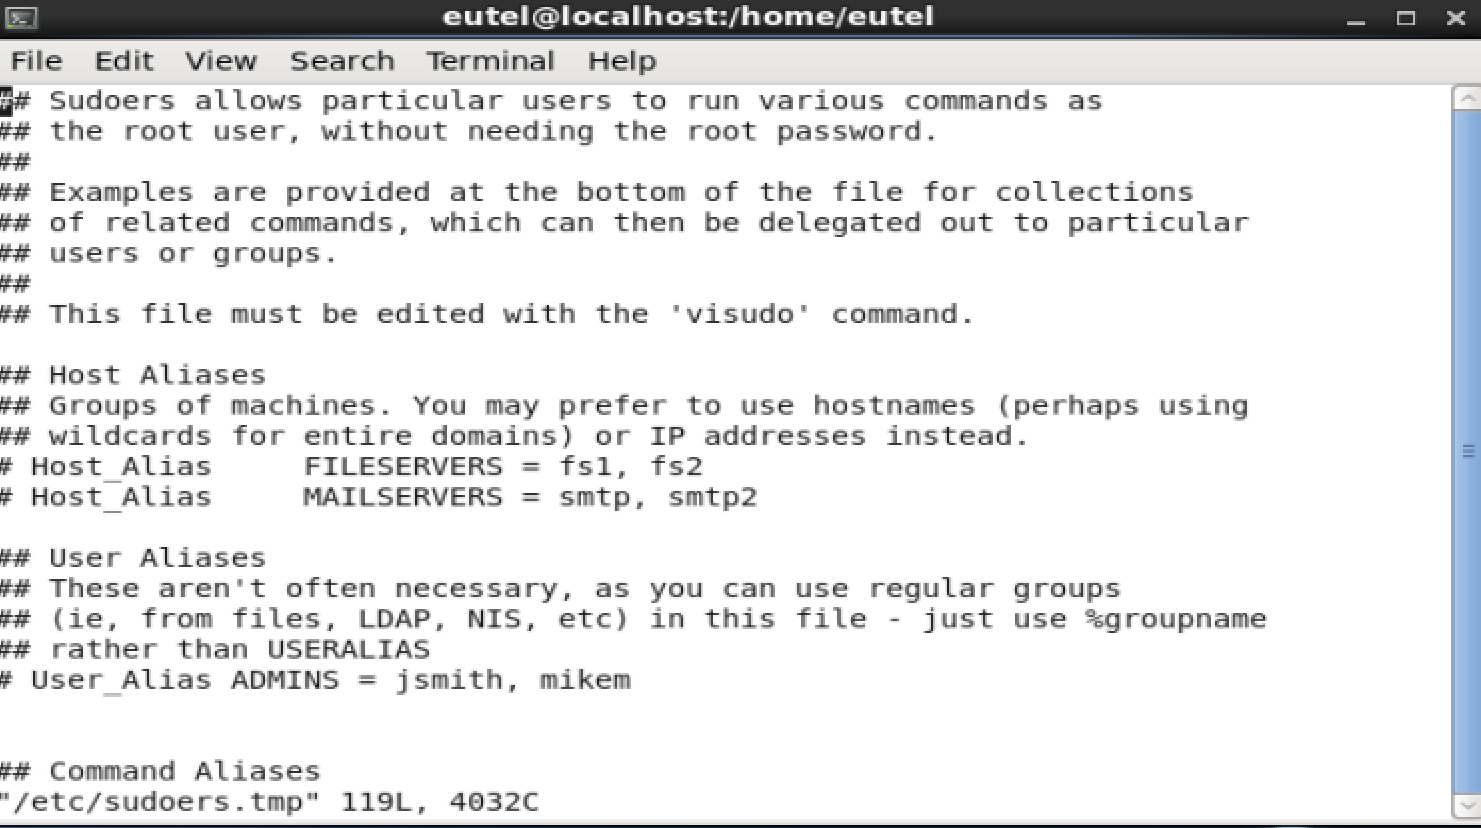
\includegraphics[scale=0.3]{visudo1.png}
	\caption{\textit{The sudoers file.}}
\end{figure}
Scroll down through the \textit{sudoers} file until you reach the commands section, and you will see the following:
\begin{figure}[!ht]
	\centering
	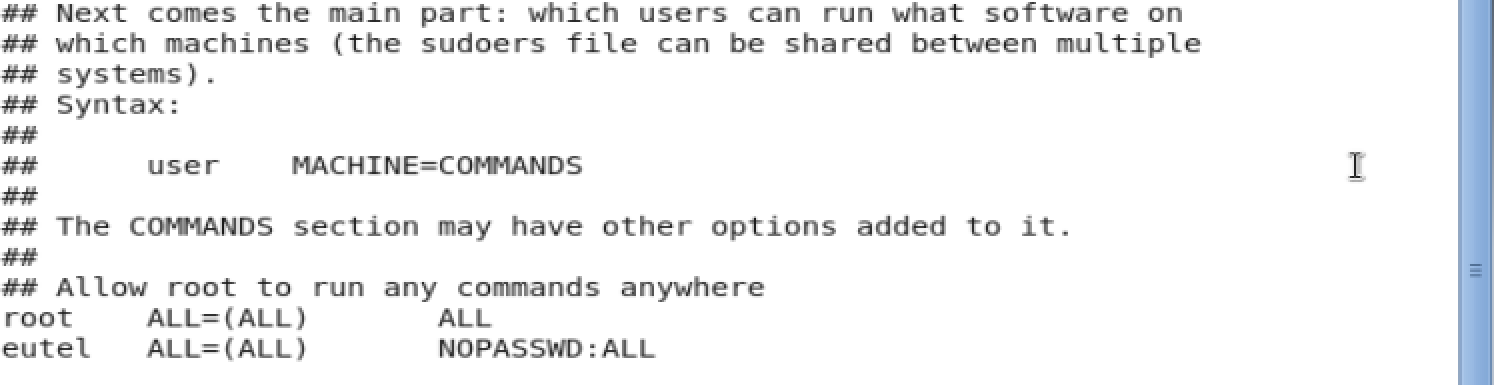
\includegraphics[scale=0.3]{visudo2.png}
	\caption{\textit{The sudoers file: command section.}}
\end{figure}
\\Locate the following line:
\begin{minted}[breaklines]{bash}
eutel	ALL=(ALL)	NOPASSWD:ALL
\end{minted}
and change it to:
\begin{minted}[breaklines]{bash}
eutel	ALL=(ALL)	ALL
\end{minted}
This will then mean that the eutel user must now enter their password when executing commands with sudo.
\paragraph{}
Note that \textit{visudo} uses vi, by default, to edit the sudoers file. If you are not familiar with how to operate vi, then you must type ``i'' before you can type, to enter ``insert'' mode. Once you are in insert mode you can then type as normal. When you are done typing and making your changes, hit ``esc'', followed by ``:x'' to save your changes and quit. For more information on the sudoers file and what it can do, visit \url{https://www.garron.me/en/linux/visudo-command-sudoers-file-sudo-default-editor.html}.
\subsection{Enabling bidirectional copy and paste}
\paragraph{}
It is highly recommended that the users of the VMs enable a bidirectional clipboard between the host and the guest. This means that the user will be able to copy and paste, in both directions, between the host and the guest machines. To do this, first ensure that the VM you wish to enable this for is shutdown. Then select the desired VM from the VM pane of the VirtualBox main window, and then click the ``settings'' button above it.
\begin{figure}[!ht]
	\centering
	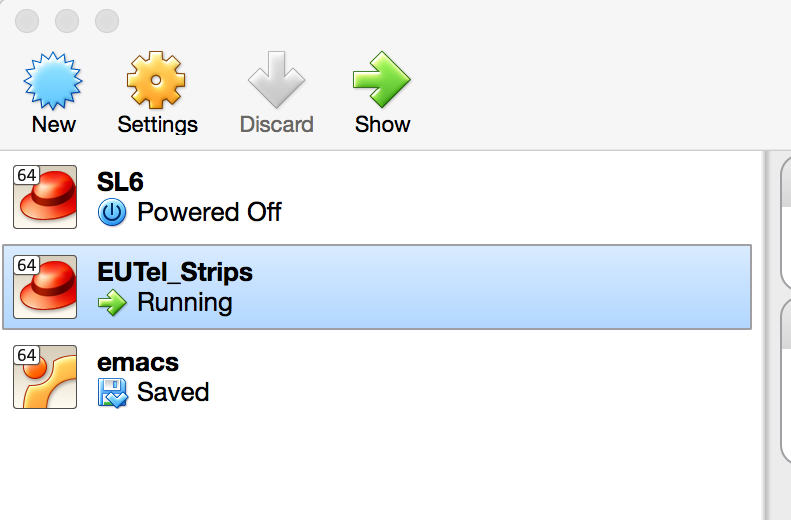
\includegraphics[scale=0.4]{copypaste1.png}
	\caption{\textit{The VM pane of the VirtualBox main window.}}
\end{figure}
In settings, navigate to the \textit{General - Advanced} tab and change the fields \textit{Shared Clipboard} and \textit{Drag 'n' Drop} to \textit{Bidirectional}. This also enables the user to drag and drop files between the host and guest.
\begin{figure}[!ht]
	\centering
	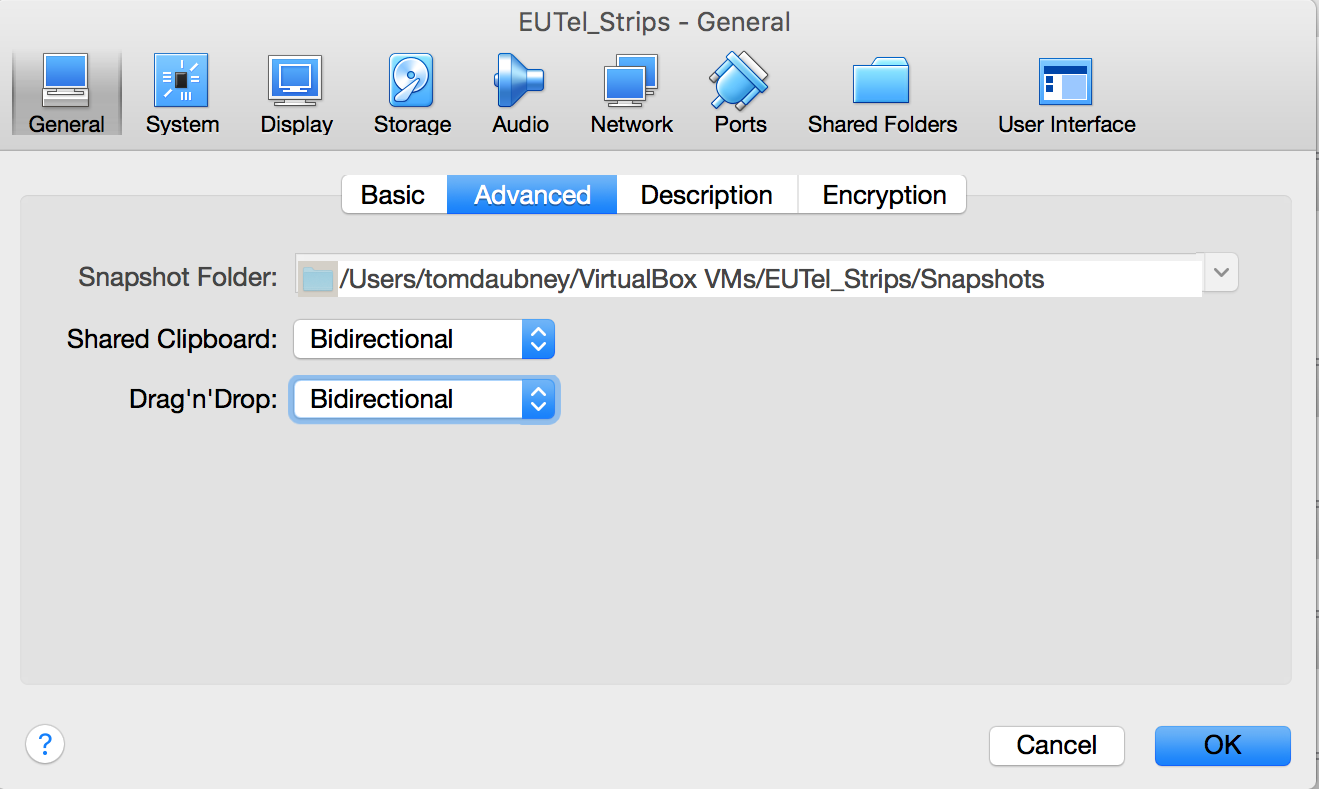
\includegraphics[scale=0.3]{copypaste2.png}
	\caption{\textit{The Advanced tab in general settings.}}
\end{figure}
\subsection{CMake v3.5.2 - EUTel\_Strips only}
\paragraph{}
In order to compile the later version of EUDAQ, CMake version 3.5.2 was installed on the virtual machine. This can be found at: /home/eutel/software/cmake-3.5.2. This was only installed on the EUTel\_Strips machine because the other VM does not have such a recent EUDAQ version installed.
\section{Docker}
\paragraph{Coming soon...}
As an alternative to virtualisation, the EUTelescope development team are planning to release an EUTelescope Dockerfile as the new version of EUTelescope becomes available. This guide will be updated in due course to provide information on how to work with Docker.
\section{Miscellaneous Tips}
\paragraph{Seeing all available processors}
To get an idea of what processors are available to you as an EUTelescope user, the easiest thing to do is navigate to the \textit{src} folder in the EUTelescope base directory. In this folder you will the source code for the project. All EUTelescope processors are a \textit{.cpp} file with the filename prefix ``EUTelescopeProcessor''. Take a look into these files to get an understanding of what the processors do.
\paragraph{Issues with memory leaks in GBLTrackFit Processor} It was noticed that a memory leak exists in \textit{src/EUTelProcessorGBLTrackFit.cpp}. In order to correct this memory leak, look for the line:
\begin{minted}[breaklines]{bash}
gbl::GblTrajectory* traj = 0;
\end{minted}
You will notice that it is defined inside a for-loop. Navigate to the closing brace of this for-loop and add:
\begin{minted}[breaklines]{bash}
delete traj;
\end{minted}
inside the loop. This should solve the error relating to the memory leaks.
\section{Troubleshooting}
\subsection{Common Problems}
\paragraph{GSL Errors}
A frequently missing library, that is required for installation is the GSL library. If your installation is halted by an error message indicating that the GSL libraries cannot be found, then please navigate to the \textit{Ubuntu Software Center}. Once there, search for GSL and download:
\begin{itemize}
	\item \textit{gsl-bin}
    \item \textit{gsl0-dev}.
\end{itemize}
Upon installing these libraries, the installation should run past the GSL error message.
\paragraph{Failed to download ROOT source}
Part of the installation of EUTelescope involves compiling ROOT. This is a cumbersome step and it is prone to causing fatal errors to the installation. If the installation script throws an error stating that the ROOT source cannot be downloaded then this can be overcome by symbolically linking an existing installation of ROOT into the directory that EUTelescope searches for ROOT.
\paragraph{}
For example, at DESY, there is a lot of software available on the AFS. Below is shown the steps needed to rectify the problem of the ROOT source not downloading here at DESY, and so only slight modifications should be needed to rectify this problem for those not at DESY.
\paragraph{}
First, navigate to:
\begin{minted}[breaklines]{bash}
ilcsoft/v01-17-05/root
\end{minted}
This directory should be created after trying to run the install script, even after it fails to download \textit{ROOT}. Once here, a tarball should be visible. Delete that tarball and add a symbolic link to an existing version of \textit{ROOT}. For example:
\begin{minted}[breaklines]{bash}
ln -s /the/directory/of/your/existing/installation/
\end{minted}
For those at DESY, this location can be used:
\begin{minted}[breaklines]{bash}
ln -s /afs/desy.de/project/ilcsoft/sw/x86_64_gcc48_ub1404/root/5.34.30
\end{minted}
Once you have done this, you \textbf{must} modify the \textit{ROOT} version number in \textit{release-versions.py} so that it matches the version of \textit{ROOT} that you have just linked to. After this, try rerunning the install script, and hopefully the problem should be solved.
\subsection{Support}
\paragraph{}
If you find an a bug within EUTelescope, please make sure you log it on the issue tracker, so the developers can take care of it. Please find the issue tracker at the following link:
\url{https://github.com/eutelescope/eutelescope/issues}
\paragraph{}
The development team will try to get back to you quickly.



\newpage
\begin{thebibliography}{9}
\bibitem{}
\url{http://eutelescope.web.cern.ch/content/about-eutelescope}
\bibitem{}
\url{http://eutelescope.web.cern.ch/content/raida-processor}
\bibitem{}
\url{http://eutelescope.web.cern.ch/content/lcio-data-format}
\bibitem{}
\url{http://eutelescope.web.cern.ch/content/gear-telescope-geometry-description}
\bibitem{}
\url{http://eutelescope.web.cern.ch/content/installation}
\bibitem{}
\url{http://eutelescope.web.cern.ch/content/steering-files}
\bibitem{}
\url{http://ilcsoft.desy.de/portal/software_packages/}
\bibitem{}
\url{http://ilcsoft.desy.de/Marlin/current/doc/html/index.html}
\bibitem{}
\url{http://eutelescope.web.cern.ch/content/job-submission}
\bibitem{}
A brief introduction to ILCSoft: LCIO, Marlin, Mokka \& Druid by Manqi.
\url{http://indico.ihep.ac.cn/event/4287/contribution/2/material/slides/0.pdf}
\end{thebibliography}
\end{document}
